% filepath: /gpfs/mcc/HT04543/jxc06/jxc74-jxc06/projects/FusionComputingLab/PhaseV_FCL1/codes/U-Net-LES/Paper_Germano_GenerativeAI.tex
\documentclass[authoryear,preprint,review,12pt]{elsarticle}

\usepackage[a4paper,margin=2cm]{geometry}
\usepackage{amsmath,amssymb}
\usepackage{graphicx}
\usepackage{hyperref}
\usepackage{booktabs}
\usepackage{subcaption}
\usepackage{algorithm}
\usepackage{algorithmic}

\hypersetup{colorlinks=true,linkcolor=black,citecolor=black,urlcolor=cyan}

\journal{Computer Physics Communications}

\begin{document}

\begin{frontmatter}

\title{Learning Germano-filtered DNS fields via Generative AI to accelerate edge plasma turbulence simulations}

\author[Hartree]{Jony Castagna}

\affiliation[Hartree]{
  organization={UKRI-STFC Hartree Centre},
  addressline={Keckwick Lane},
  city={Daresbury},
  postcode={WA4 4AD},
  country={United Kingdom}
}

\begin{abstract}
High-fidelity simulations of edge-plasma turbulence are computationally expensive because the dynamically relevant scales span several orders of magnitude. Large Eddy Simulation (LES) reduces this cost by filtering the governing equations, but requires a closure for the unresolved nonlinear terms. In this work, we investigate a generative-AI closure based on learning DNS fields filtered according to the Germano formalism. The method reconstructs fine-scale density and electrostatic-potential fields from coarse Hasegawa--Wakatani states and evaluates the nonlinear Poisson-bracket terms on the reconstructed fields. We assess the approach using four simulation configurations: the Hasegawa-Wakatani and modified Hasegawa-Wakatani models for 256x256 and 512x512 resolutions. We compare the generative model with DNS and conventional LES diagnostics, including energy, enstrophy, spectra, probability distributions, poloidal and radial fluxes and computational cost. The supplied U-Net validation results show qualitative agreement in several integral and spectral diagnostics, but also delayed transients and excess late-time enstrophy in the modified $256^2$ case. Computational speedup remains to be quantified.
\end{abstract}

\begin{keyword}
Generative artificial intelligence \sep Large Eddy Simulation \sep
Hasegawa--Wakatani model \sep plasma turbulence \sep Germano filtering
\end{keyword}

\end{frontmatter}

\section{Introduction}

Edge-plasma turbulence strongly influences transport in magnetic-confinement fusion devices. Resolving the full range of turbulent scales with Direct Numerical Simulation (DNS) is often prohibitively expensive, particularly when long-time statistics or parameter scans are required. Reduced-resolution LES provides a practical alternative, but the filtering operation introduces unclosed nonlinear terms.

For a field $f$, the spatially filtered quantity is written as
\begin{equation}
    \widetilde{f}(\mathbf{x},t)
    =
    G \star f(\mathbf{x},t),
\end{equation}
where $G$ is a spatial filter. Filtering the nonlinear Poisson bracket produces
\begin{equation}
    \widetilde{\{\phi,f\}}
    =
    \{\widetilde{\phi},\widetilde{f}\}
    +
    \tau_{\mathrm{SGS},f},
\end{equation}
where
\begin{equation}
    \tau_{\mathrm{SGS},f}
    =
    \widetilde{\{\phi,f\}}
    -
    \{\widetilde{\phi},\widetilde{f}\}
\end{equation}
is the exact sub-grid-scale contribution.

Traditional LES closures approximate $\tau_{\mathrm{SGS},f}$ using eddy-viscosity or structural models. These approaches are inexpensive, but their accuracy can depend strongly on the filter, resolution and turbulence regime. Machine-learning methods offer an alternative by learning the relationship between resolved and unresolved structures directly from high-fidelity data.

Generative adversarial networks (GANs) are particularly attractive because they can generate spatially coherent fine-scale fields. Rather than predicting the sub-grid term directly, the present approach learns a DNS field whose filtered representation agrees with the LES state. The reconstructed field is then used to evaluate the nonlinear terms. This preserves the structure of the governing equations while replacing the explicit closure model with a learned deconvolution operator.

The method is tested on the Hasegawa--Wakatani (HW) system and its modified form. The simulations are represented by the four cases
\begin{center}
\texttt{HW\_N256}, \quad
\texttt{HW\_N512}, \quad
\texttt{mHW\_N256}, \quad
\texttt{mHW\_N512}.
\end{center}
The objectives are to:

\begin{enumerate}
    \item quantify the accuracy of the learned reconstruction;
    \item compare standard and modified HW turbulence;
    \item assess the effect of spatial resolution;
    \item compare generative-AI LES with DNS and conventional LES;
    \item measure the computational cost and achievable speedup.
\end{enumerate}

\section{Physical model}

The normalized two-dimensional Hasegawa--Wakatani equations are
\begin{align}
    \frac{\partial \zeta}{\partial t}
    + \{\phi,\zeta\}
    &=
    -\alpha(\phi-n)
    + \nu_\zeta\nabla^2\zeta,
    \label{eq:hw_vorticity}
    \\
    \frac{\partial n}{\partial t}
    + \{\phi,n\}
    &=
    -\alpha(\phi-n)
    - k\frac{\partial\phi}{\partial y}
    + \nu_n\nabla^2n,
    \label{eq:hw_density}
\end{align}
where $n$ is the density fluctuation, $\phi$ is the electrostatic potential and
\begin{equation}
    \zeta=\nabla^2\phi
\end{equation}
is the vorticity. The Poisson bracket is
\begin{equation}
    \{a,b\}
    =
    \frac{\partial a}{\partial x}
    \frac{\partial b}{\partial y}
    -
    \frac{\partial a}{\partial y}
    \frac{\partial b}{\partial x}.
\end{equation}

Here, $\alpha$ is the adiabatic parameter, $k$ is the background density-gradient coefficient, and $\nu_\zeta$ and $\nu_n$ are diffusion coefficients.

The modified Hasegawa--Wakatani model used in the simulations is written generically as
\begin{align}
    \frac{\partial \zeta}{\partial t}
    + \{\phi,\zeta\}
    &=
    \mathcal{R}_{\zeta}(\phi,n)
    + \nu_\zeta\nabla^2\zeta,
    \\
    \frac{\partial n}{\partial t}
    + \{\phi,n\}
    &=
    \mathcal{R}_{n}(\phi,n)
    - k\frac{\partial\phi}{\partial y}
    + \nu_n\nabla^2n,
\end{align}
where $\mathcal{R}_{\zeta}$ and $\mathcal{R}_{n}$ denote the modified resistive coupling implemented in the BOUT++ input files.

\section{Germano-filtered LES formulation}

Applying a filter to Eqs.~\eqref{eq:hw_vorticity}--\eqref{eq:hw_density} gives
\begin{align}
    \frac{\partial\widetilde{\zeta}}{\partial t}
    + \{\widetilde{\phi},\widetilde{\zeta}\}
    &=
    -\alpha(\widetilde{\phi}-\widetilde{n})
    -\tau_{\mathrm{SGS},\zeta}
    +\nu_\zeta\nabla^2\widetilde{\zeta},
    \\
    \frac{\partial\widetilde{n}}{\partial t}
    + \{\widetilde{\phi},\widetilde{n}\}
    &=
    -\alpha(\widetilde{\phi}-\widetilde{n})
    -\tau_{\mathrm{SGS},n}
    -k\frac{\partial\widetilde{\phi}}{\partial y}
    +\nu_n\nabla^2\widetilde{n}.
\end{align}

The exact closure terms are obtained from paired DNS and filtered DNS fields:
\begin{align}
    \tau_{\mathrm{SGS},\zeta}
    &=
    \widetilde{\{\phi,\zeta\}}
    -
    \{\widetilde{\phi},\widetilde{\zeta}\},
    \\
    \tau_{\mathrm{SGS},n}
    &=
    \widetilde{\{\phi,n\}}
    -
    \{\widetilde{\phi},\widetilde{n}\}.
\end{align}

Following the Germano procedure, a second test filter may be applied to separate the resolved and unresolved contributions. In the present work, the filtered DNS fields are used as training targets, while the generative model learns the inverse mapping
\begin{equation}
    \mathcal{G}:
    (\widetilde{n},\widetilde{\phi})
    \longrightarrow
    (n^{\mathrm{GAN}},\phi^{\mathrm{GAN}}).
\end{equation}

The generated vorticity is obtained consistently from the generated potential:
\begin{equation}
    \zeta^{\mathrm{GAN}}
    =
    \nabla^2\phi^{\mathrm{GAN}}.
\end{equation}
This avoids independently generating a vorticity field that may be inconsistent with $\phi$.

\section{Generative-AI reconstruction}

The generator is trained using DNS fields and their corresponding Germano-filtered fields. The reconstruction loss is
\begin{equation}
    \mathcal{L}_{\mathrm{rec}}
    =
    \left\|
    G\star\mathbf{U}^{\mathrm{GAN}}_{\mathrm{DNS}}
    -
    \mathbf{U}_{\mathrm{LES}}
    \right\|_2^2,
\end{equation}
where
\begin{equation}
    \mathbf{U}=(n,\phi,\zeta).
\end{equation}

To improve statistical agreement, the loss can be supplemented by gradient and spectral terms:
\begin{equation}
    \mathcal{L}
    =
    \lambda_{\mathrm{rec}}\mathcal{L}_{\mathrm{rec}}
    +
    \lambda_{\nabla}\mathcal{L}_{\nabla}
    +
    \lambda_{\mathrm{spec}}\mathcal{L}_{\mathrm{spec}}
    +
    \lambda_{\mathrm{adv}}\mathcal{L}_{\mathrm{adv}}.
\end{equation}

The LES time integration proceeds as follows:

\begin{enumerate}
    \item advance the coarse HW state;
    \item normalize the LES input fields;
    \item reconstruct the DNS-resolution fields using the generator;
    \item calculate $\zeta^{\mathrm{GAN}}=\nabla^2\phi^{\mathrm{GAN}}$;
    \item evaluate the nonlinear Poisson brackets;
    \item filter the nonlinear terms;
    \item advance the filtered equations.
\end{enumerate}

\section{Numerical dataset}

The data were generated with the BOUT++ Hasegawa--Wakatani implementation. Four configurations were analysed:

\begin{table}[ht]
\centering
\caption{Simulation cases analysed in this work. Values marked TODO should be extracted from the corresponding BOUT++ output files.}
\label{tab:cases}
\begin{tabular}{llllll}
\toprule
Case & Model & DNS resolution & LES resolution & $\alpha$ & Samples \\
\midrule
HW\_N256  & HW  & $256^2$ & TODO & TODO & TODO \\
HW\_N512  & HW  & $512^2$ & TODO & TODO & TODO \\
mHW\_N256 & mHW & $256^2$ & TODO & TODO & TODO \\
mHW\_N512 & mHW & $512^2$ & TODO & TODO & TODO \\
\bottomrule
\end{tabular}
\end{table}

All simulations used periodic boundary conditions. Training and validation samples were separated temporally to reduce correlation between neighbouring snapshots. The final test trajectories were not used during model optimization.

\section{Results}

The diagnostics below use the supplied U-Net validation plots for the four configurations. The numeric legend entries identify the coarse-grid sizes: 128 and 64 for the $256^2$ DNS cases, and 256, 128 and 64 for the $512^2$ DNS cases. DNS is the reference. These figures do not include a separately identified conventional LES closure or establish a comparison between adversarial and non-adversarial training. Accordingly, the plotted learned solutions are referred to as U-Net reconstructions in this section.

The $256^2$ histories extend to $t=1000$, whereas the $512^2$ histories cover approximately $t=100$. Thus, differences between these cases cannot be attributed to spatial resolution alone. The following comparisons are qualitative assessments of the archived figures; pointwise error metrics, time-averaged transport errors and timing measurements require the underlying numerical records.


\subsection{Reconstruction accuracy}

The reconstruction accuracy was evaluated using the normalized mean-square error,
\begin{equation}
    \mathrm{NMSE}(f)
    =
    \frac{\|f^{\mathrm{GAN}}-f^{\mathrm{DNS}}\|_2^2}
    {\|f^{\mathrm{DNS}}\|_2^2},
\end{equation}
the structural similarity index, and the correlation coefficient.

\begin{table}[ht]
\centering
\caption{Reconstruction metrics for the four test cases.}
\label{tab:reconstruction}
\begin{tabular}{lcccccc}
\toprule
Case & NMSE$(n)$ & NMSE$(\phi)$ & NMSE$(\zeta)$ &
SSIM$(n)$ & SSIM$(\phi)$ & SSIM$(\zeta)$ \\
\midrule
HW\_N256  & TODO & TODO & TODO & TODO & TODO & TODO \\
HW\_N512  & TODO & TODO & TODO & TODO & TODO & TODO \\
mHW\_N256 & TODO & TODO & TODO & TODO & TODO & TODO \\
mHW\_N512 & TODO & TODO & TODO & TODO & TODO & TODO \\
\bottomrule
\end{tabular}
\end{table}

The supplied diagnostic images do not determine NMSE, SSIM or fieldwise correlations; these entries remain to be evaluated from matched numerical snapshots. Statistical comparisons are presented below.

\subsection{Energy and enstrophy}

The continuum energy and generalized enstrophy are
\begin{align}
 E &= \frac12\int_\Omega\left(n^2+|\nabla\phi|^2\right)\,d\mathbf{x},\\
 W &= \frac12\int_\Omega(n-\zeta)^2\,d\mathbf{x}.
\end{align}
The supplied energy plots use the diagnostic convention
\begin{equation}
 E_{\mathrm{plot}}=\frac{L_xL_y}{2}\sum_{i,j}
 \left[n_{ij}^2+(D_x\phi)_{ij}^2+(D_y\phi)_{ij}^2\right],
\end{equation}
where $D_x$ and $D_y$ are fourth-order periodic finite-difference derivatives. This differs from the usual integral quadrature by the number of diagnostic grid points, $N_xN_y$, since $\Delta x\Delta y=L_xL_y/(N_xN_y)$. The enstrophy plots instead use
\begin{equation}
 W_{\mathrm{plot}}=\frac{\Delta x\Delta y}{2}\sum_{i,j}(n_{ij}-\zeta_{ij})^2.
\end{equation}
We retain the normalization of the supplied images. Absolute energy levels across diagnostic grids must therefore not be interpreted as directly comparable continuum integrals.

Figures~\ref{fig:energy} and~\ref{fig:enstrophy} show that the HW reconstructions retain the overall magnitude of both diagnostics, but do not track all DNS fluctuations. For HW\_N256, the 64-grid trajectory lies below DNS over substantial intervals, while the 128-grid trajectory also exhibits timing differences. For HW\_N512, the 64-grid solution has the clearest persistent deficit; the finer reconstructions remain closer but miss part of the late DNS increase.

For mHW\_N256, the initial decay is captured, but the subsequent recovery in energy and the enstrophy burst occur later in the reconstructions than in DNS. At late times, the reconstructed energy returns near the DNS level while the enstrophy remains substantially higher. Agreement in total energy alone therefore does not establish agreement in the density--vorticity diagnostic. In mHW\_N512, the 256- and 128-grid curves closely follow the energy and enstrophy decay over the shorter observation window, while the 64-grid curves show a larger deficit. This shorter window does not test the late evolution seen in mHW\_N256.

\begin{figure}[p]
\centering
\begin{subfigure}[t]{0.48\textwidth}
\centering
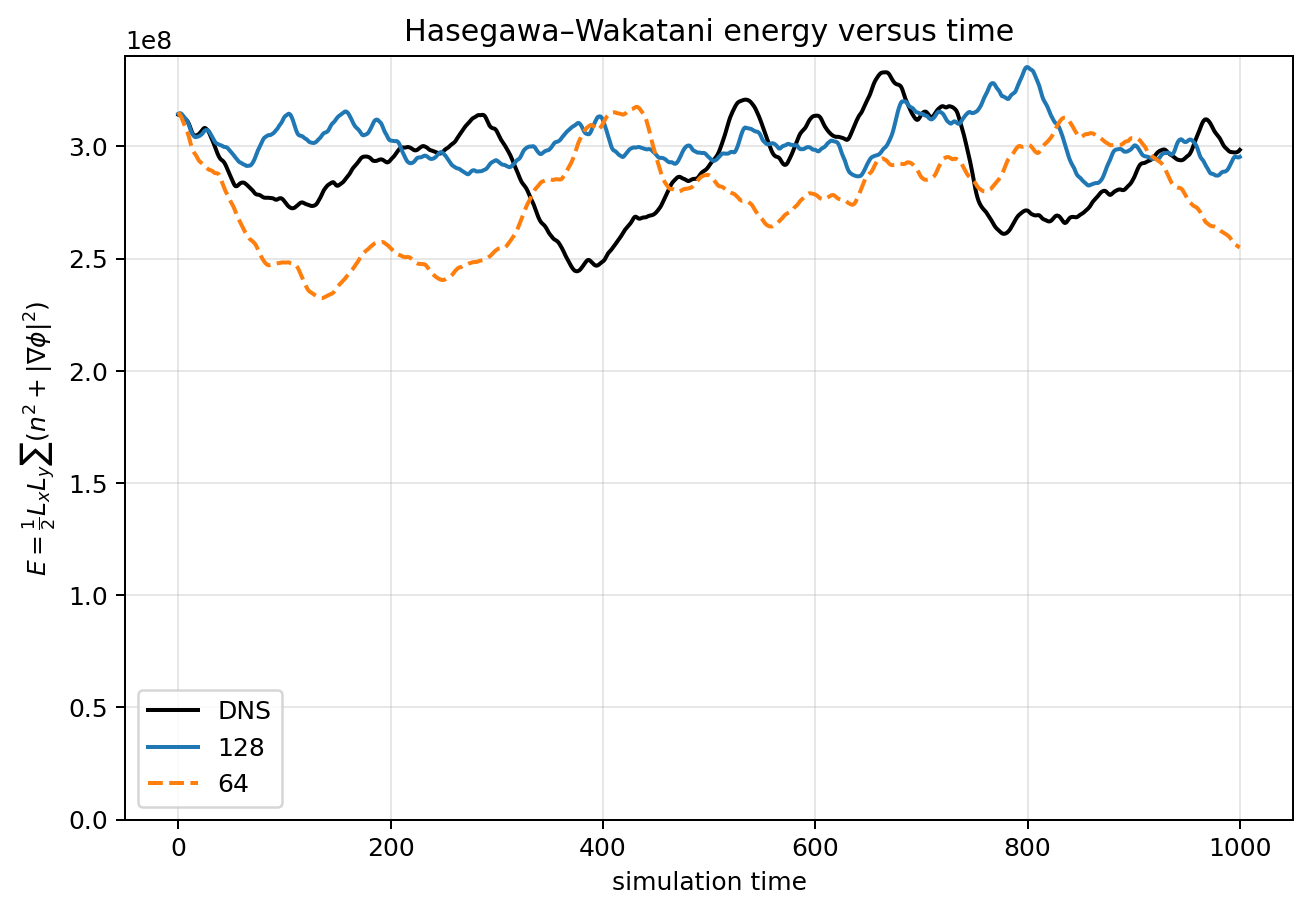
\includegraphics[width=\linewidth]{images/HW_N256_energy_vs_time.png}
\caption{\texttt{HW\_N256}}
\end{subfigure}
\hfill
\begin{subfigure}[t]{0.48\textwidth}
\centering
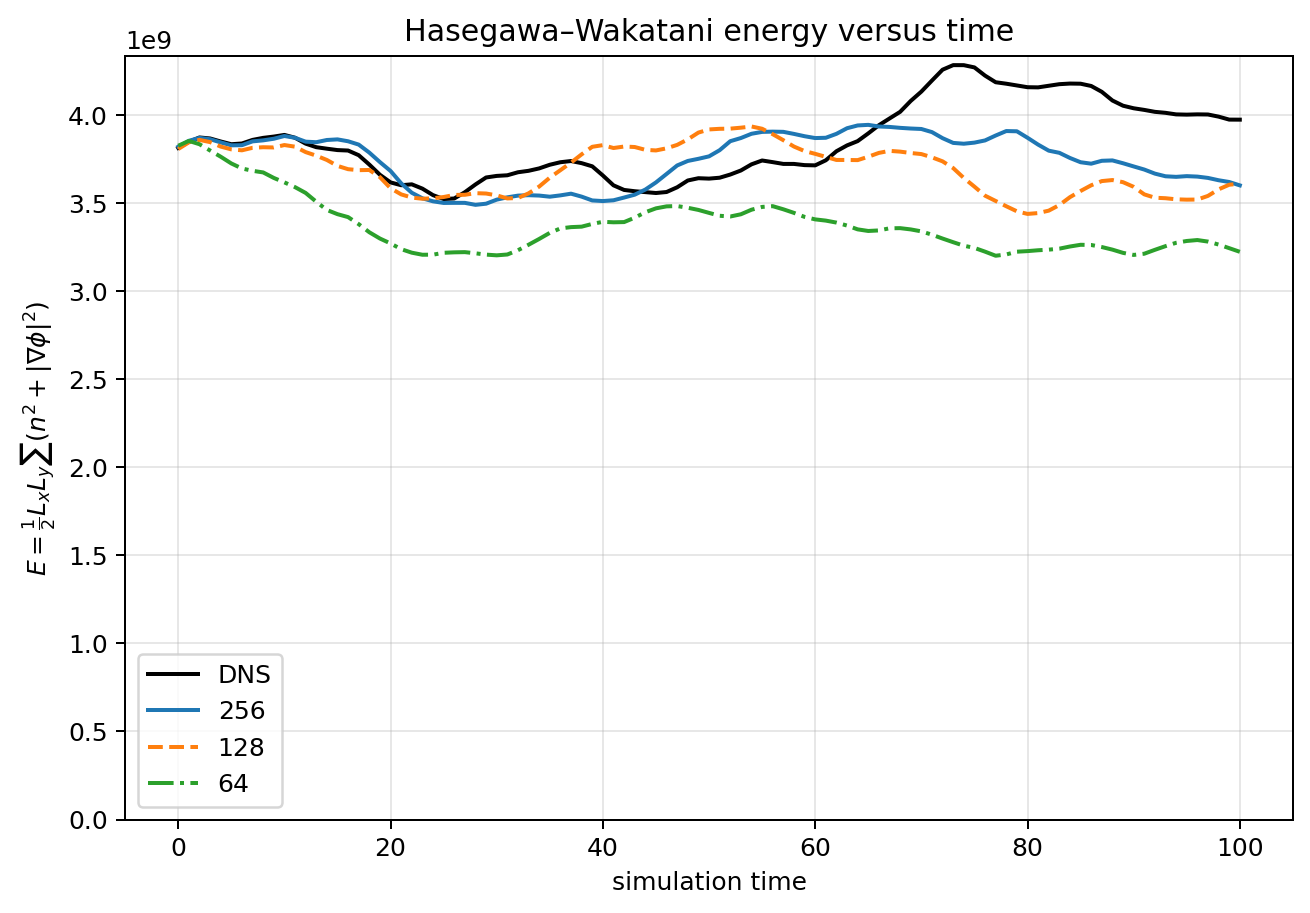
\includegraphics[width=\linewidth]{images/HW_N512_energy_vs_time.png}
\caption{\texttt{HW\_N512}}
\end{subfigure}
\par\smallskip
\begin{subfigure}[t]{0.48\textwidth}
\centering
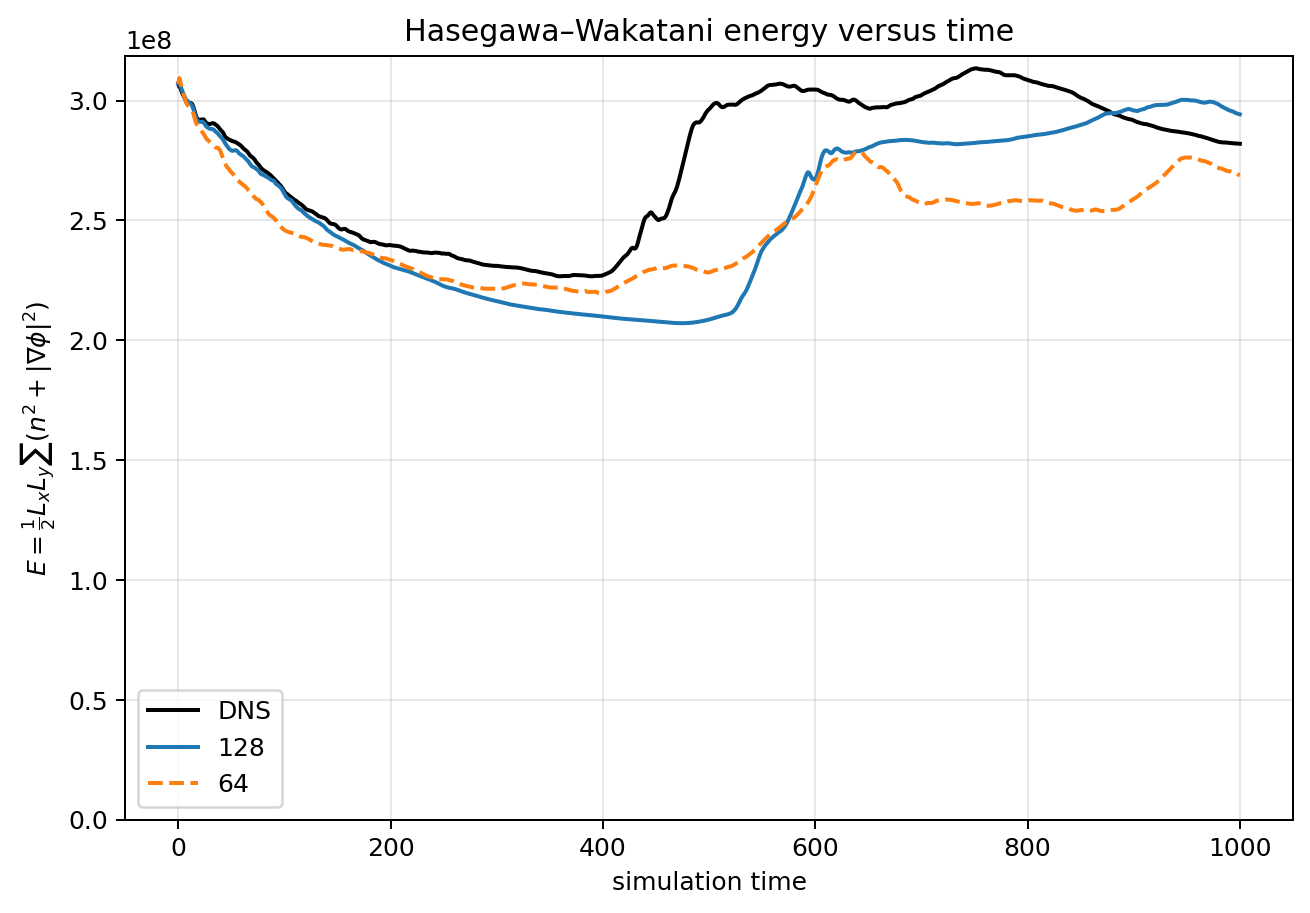
\includegraphics[width=\linewidth]{images/mHW_N256_energy_vs_time.png}
\caption{\texttt{mHW\_N256}}
\end{subfigure}
\hfill
\begin{subfigure}[t]{0.48\textwidth}
\centering
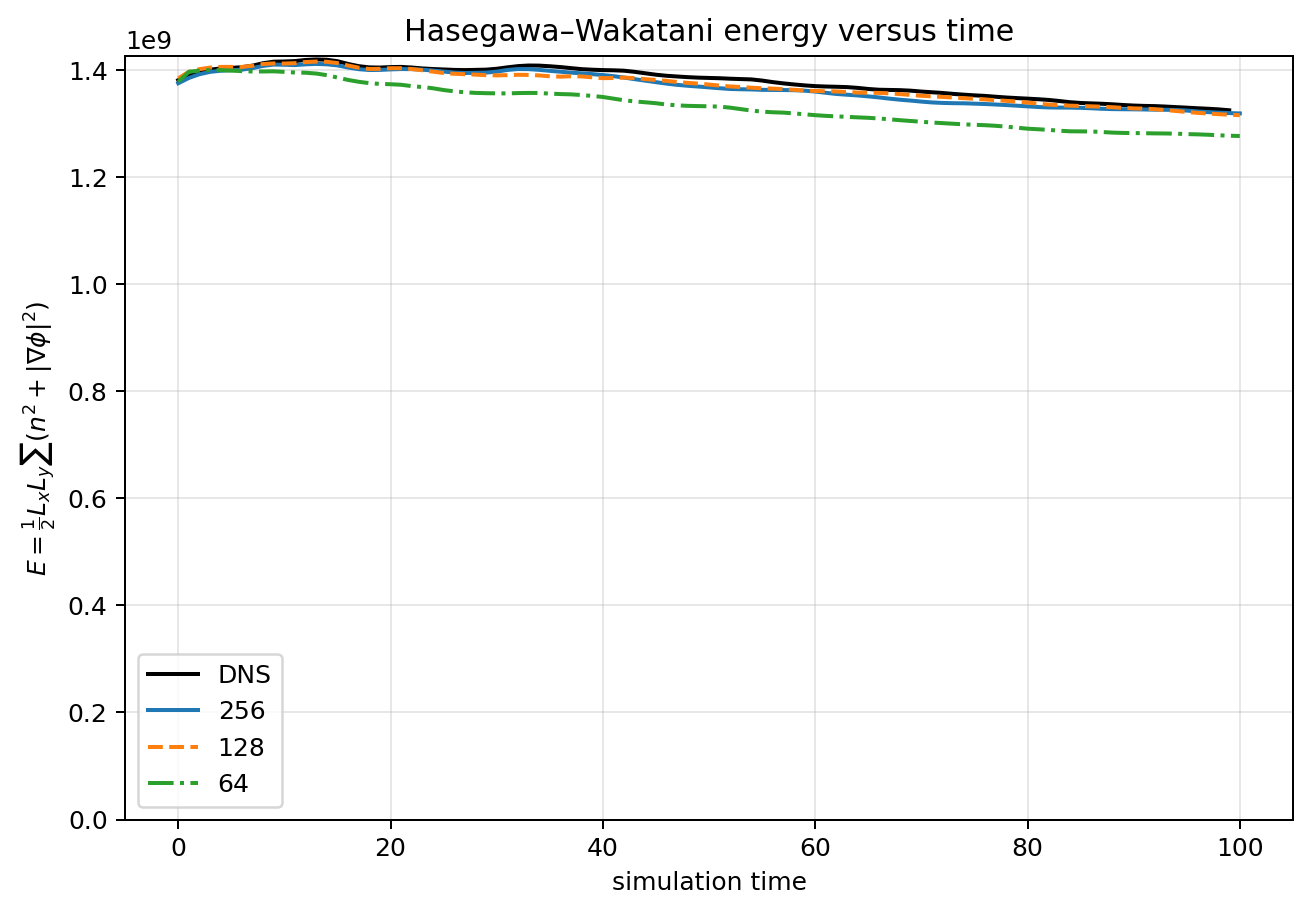
\includegraphics[width=\linewidth]{images/mHW_N512_energy_vs_time.png}
\caption{\texttt{mHW\_N512}}
\end{subfigure}
\caption{Energy histories using the $E_{\mathrm{plot}}$ normalization defined in the text. Each panel compares DNS with the coarse-grid sizes listed in its legend. The observation interval differs between the $256^2$ and $512^2$ cases.}
\label{fig:energy}
\end{figure}
\begin{figure}[p]
\centering
\begin{subfigure}[t]{0.48\textwidth}
\centering
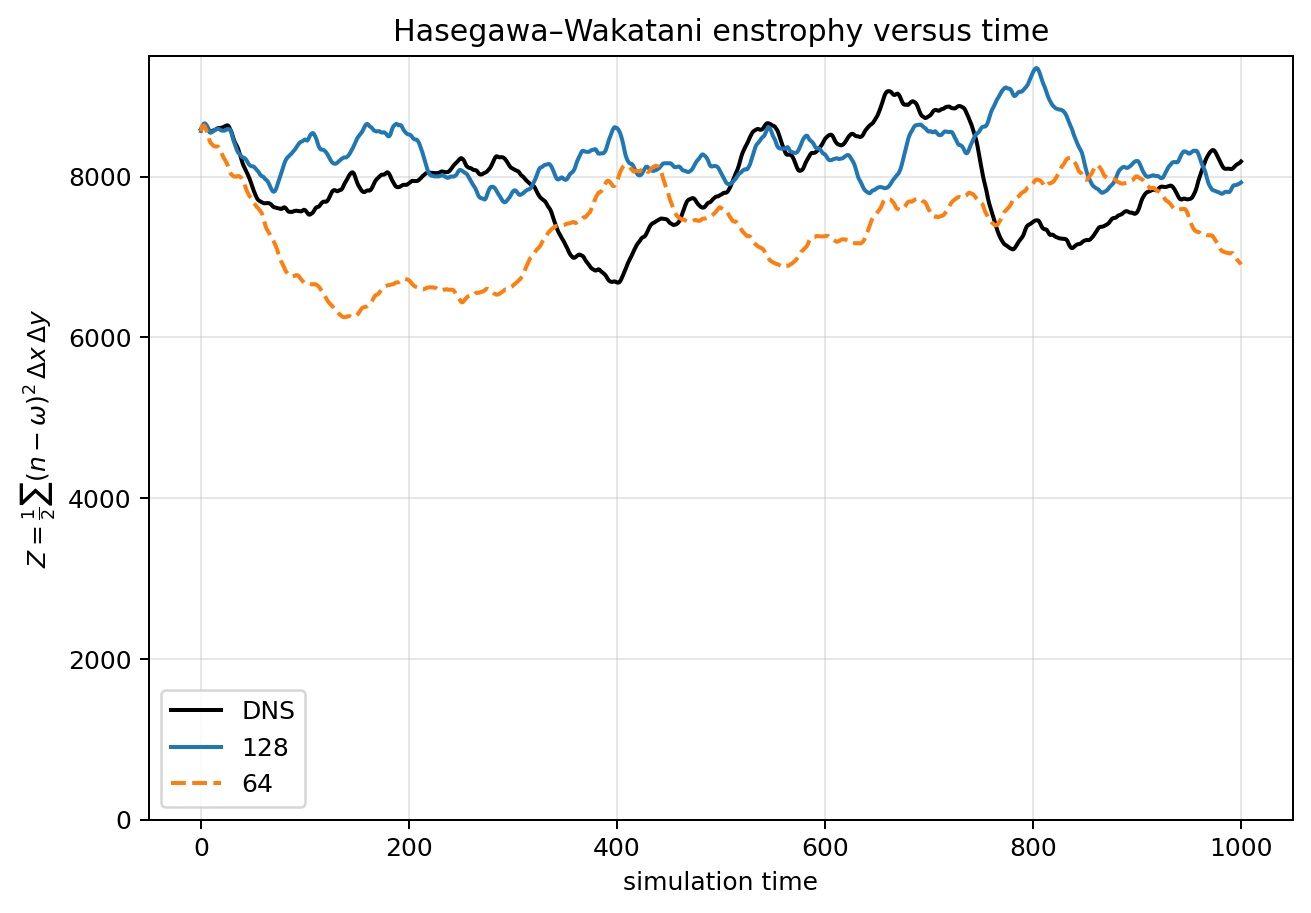
\includegraphics[width=\linewidth]{images/HW_N256_enstrophy_vs_time.png}
\caption{\texttt{HW\_N256}}
\end{subfigure}
\hfill
\begin{subfigure}[t]{0.48\textwidth}
\centering
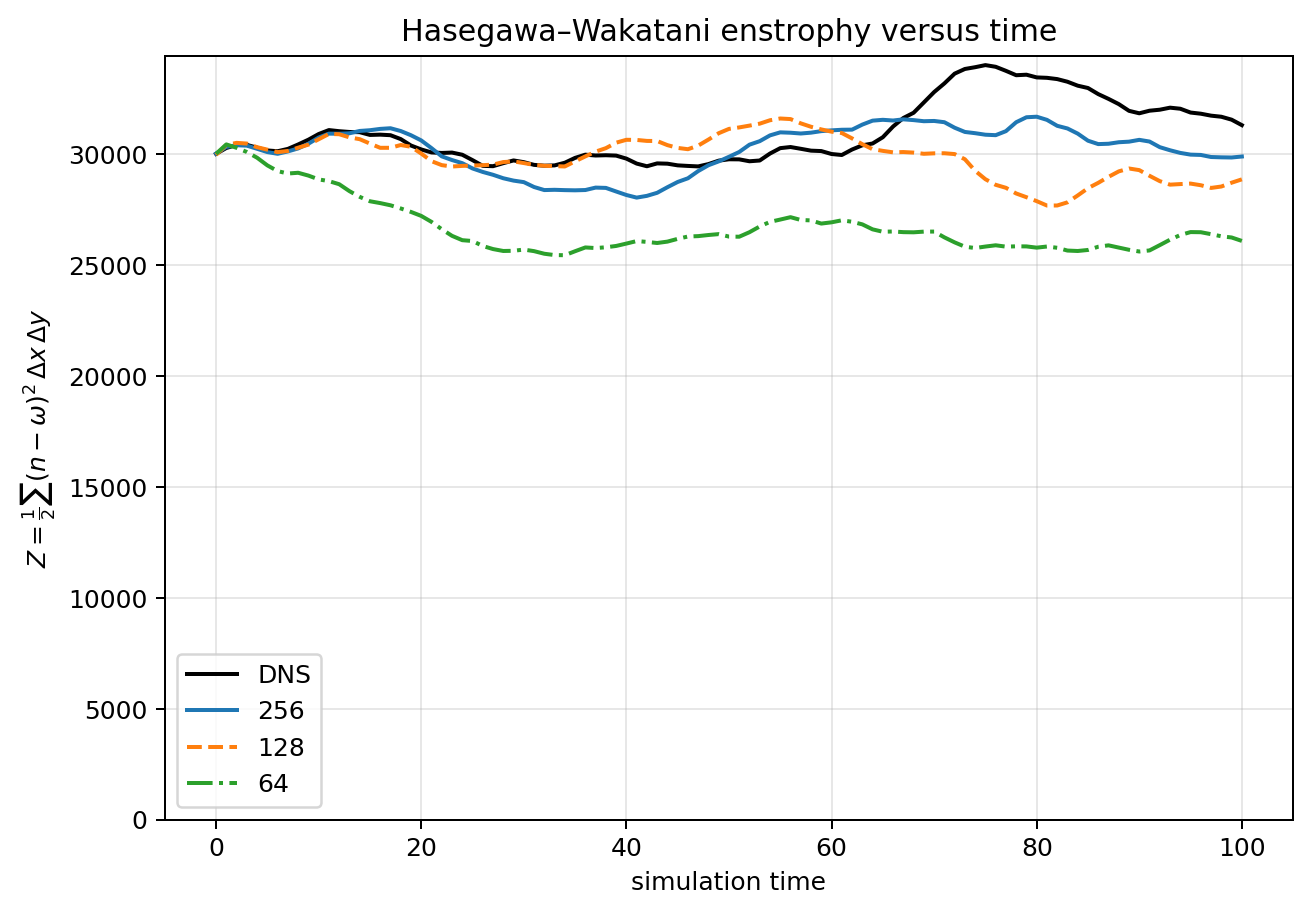
\includegraphics[width=\linewidth]{images/HW_N512_enstrophy_vs_time.png}
\caption{\texttt{HW\_N512}}
\end{subfigure}
\par\smallskip
\begin{subfigure}[t]{0.48\textwidth}
\centering
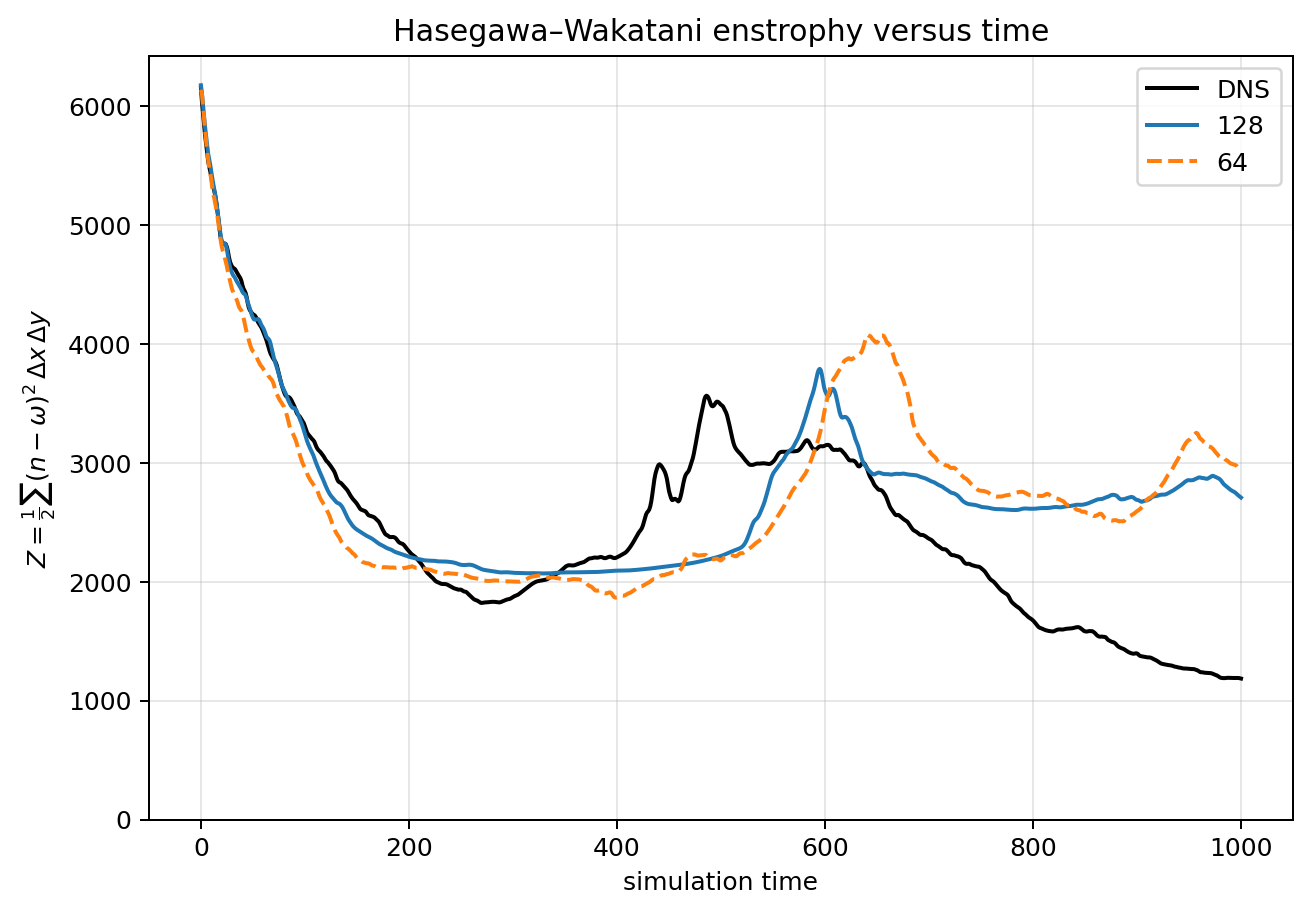
\includegraphics[width=\linewidth]{images/mHW_N256_enstrophy_vs_time.png}
\caption{\texttt{mHW\_N256}}
\end{subfigure}
\hfill
\begin{subfigure}[t]{0.48\textwidth}
\centering
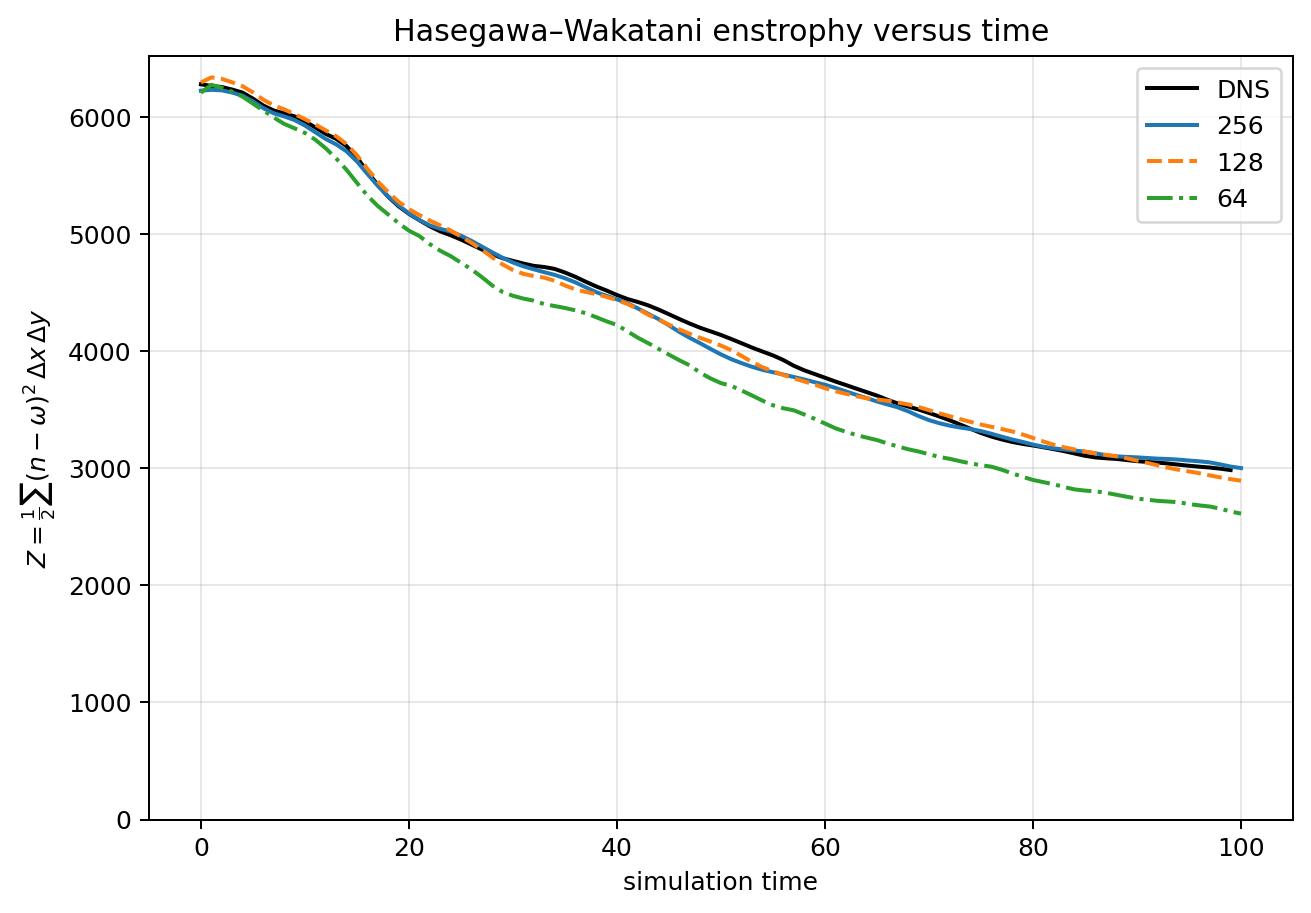
\includegraphics[width=\linewidth]{images/mHW_N512_enstrophy_vs_time.png}
\caption{\texttt{mHW\_N512}}
\end{subfigure}
\caption{Generalized enstrophy histories, $W_{\mathrm{plot}}=\frac12\Delta x\Delta y\sum(n-\zeta)^2$. The delayed transient and elevated late-time enstrophy in mHW\_N256 contrast with the closer agreement over the shorter mHW\_N512 interval.}
\label{fig:enstrophy}
\end{figure}

\subsection{Spectral statistics}

The archived spectra are shell sums of the total HW energy, including both density and potential-gradient contributions, rather than kinetic energy alone:
\begin{equation}
 E(k_s)=\frac12\sum_{\mathbf{k}\in\mathcal{S}_s}
 \left(|\widehat n_{\mathbf{k}}|^2+|\mathbf{k}|^2|\widehat\phi_{\mathbf{k}}|^2\right),
\end{equation}
where the Fourier coefficients are normalized by $N_xN_y$ and $\mathcal{S}_s$ denotes a radial wavenumber shell. This spectral normalization is distinct from that of $E_{\mathrm{plot}}$.

Figure~\ref{fig:spectra} includes all three available initial/final spectrum images. No corresponding initial/final image is present for HW\_N512, so no final-spectrum conclusion is drawn for that case. Initial spectra nearly overlap over the energetic scales. At the final time, HW\_N256 retains a similar spectral shape, with differences at the lowest wavenumbers and in the dissipative tail. For mHW\_N256, the reconstructions retain more high-wavenumber energy than DNS, consistent with the elevated late-time enstrophy. For mHW\_N512, agreement is close over the energetic scales, but the reconstructed tails depart from DNS at high wavenumbers. The vertical reference marks the 64-grid Nyquist wavenumber, not a measured boundary of accurate reconstruction.

\begin{figure}[p]
\centering
\begin{subfigure}[t]{0.98\textwidth}
\centering
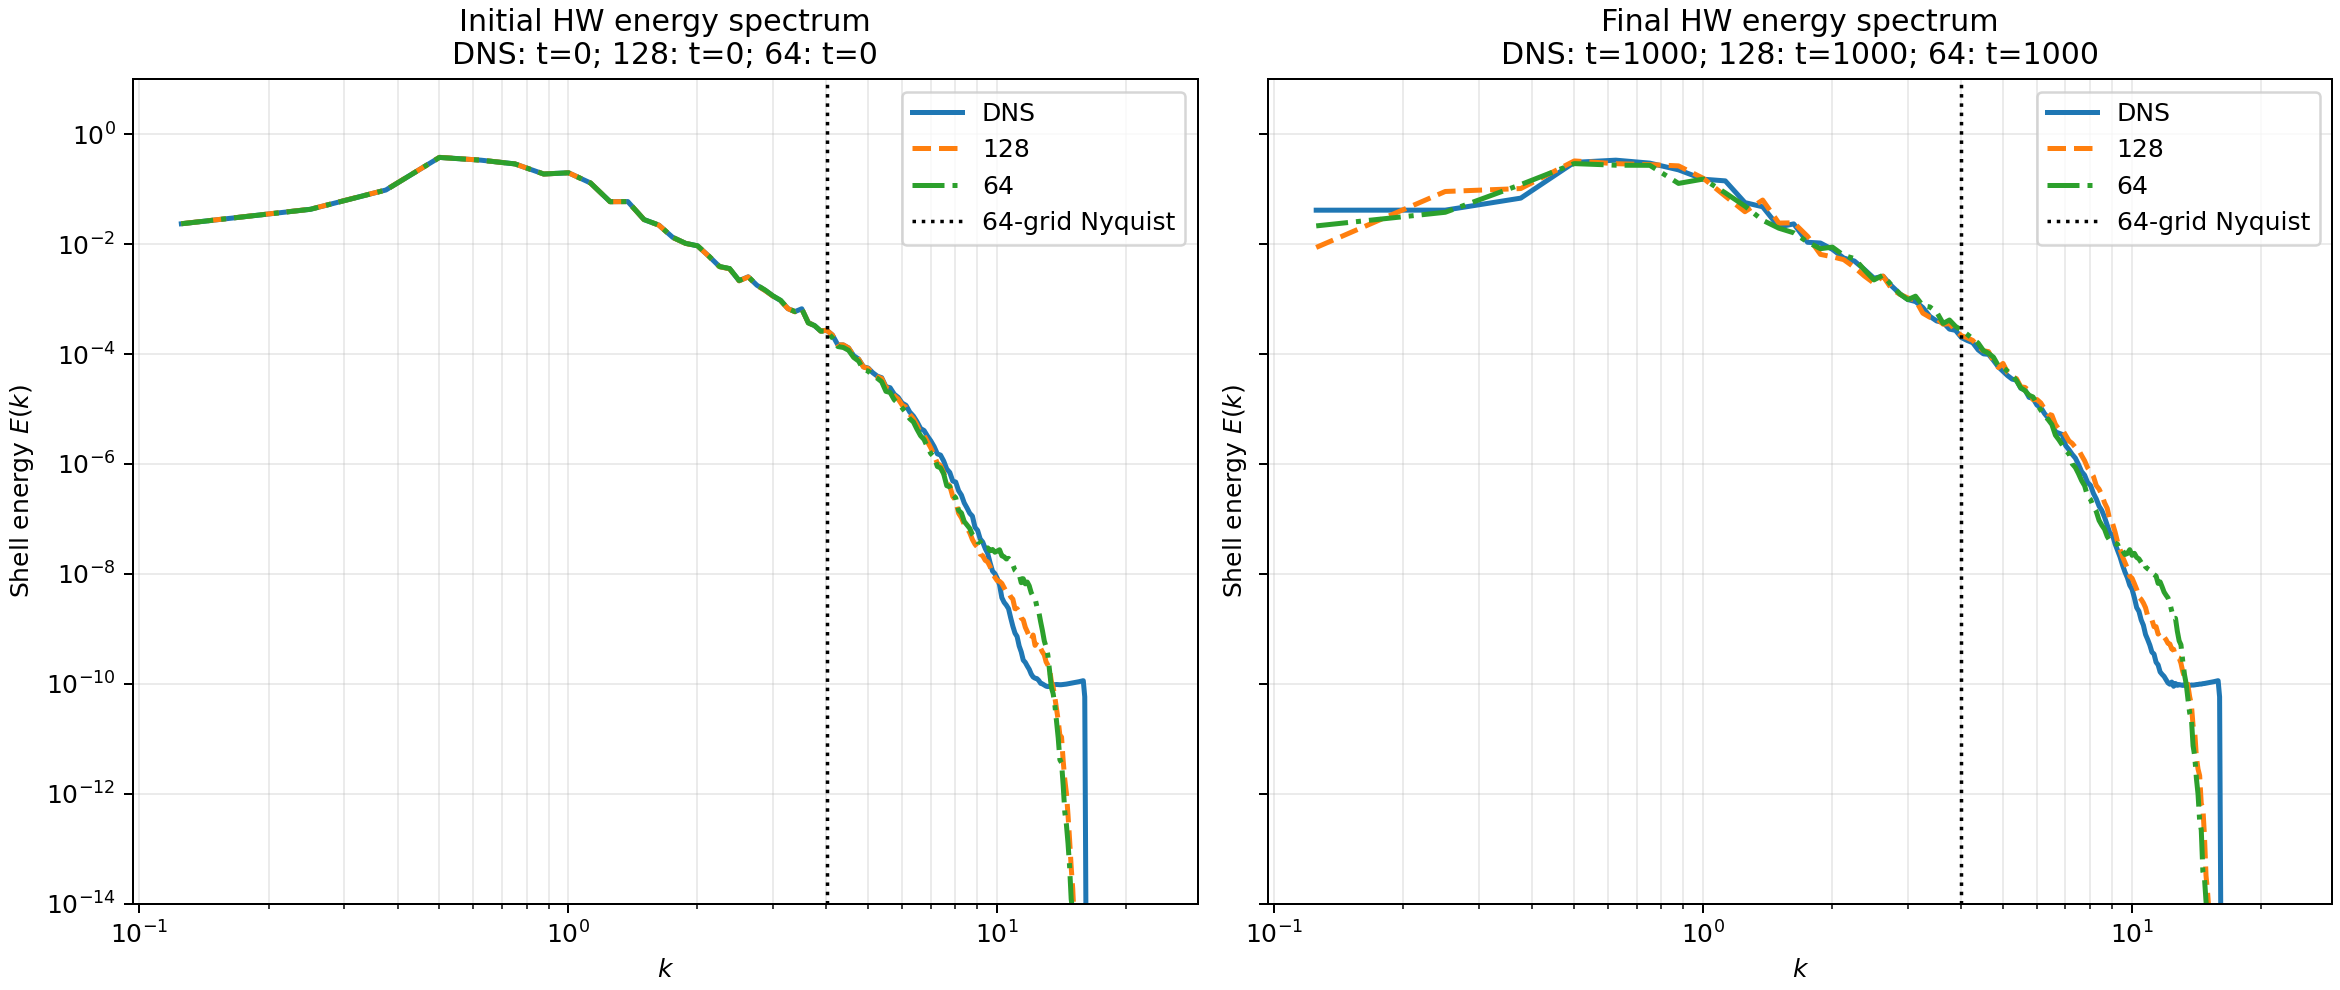
\includegraphics[width=\linewidth,height=0.235\textheight,keepaspectratio]{images/HW_N256_hw_energy_spectra_initial_final.png}
\caption{\texttt{HW\_N256}}
\end{subfigure}
\par\smallskip
\begin{subfigure}[t]{0.98\textwidth}
\centering
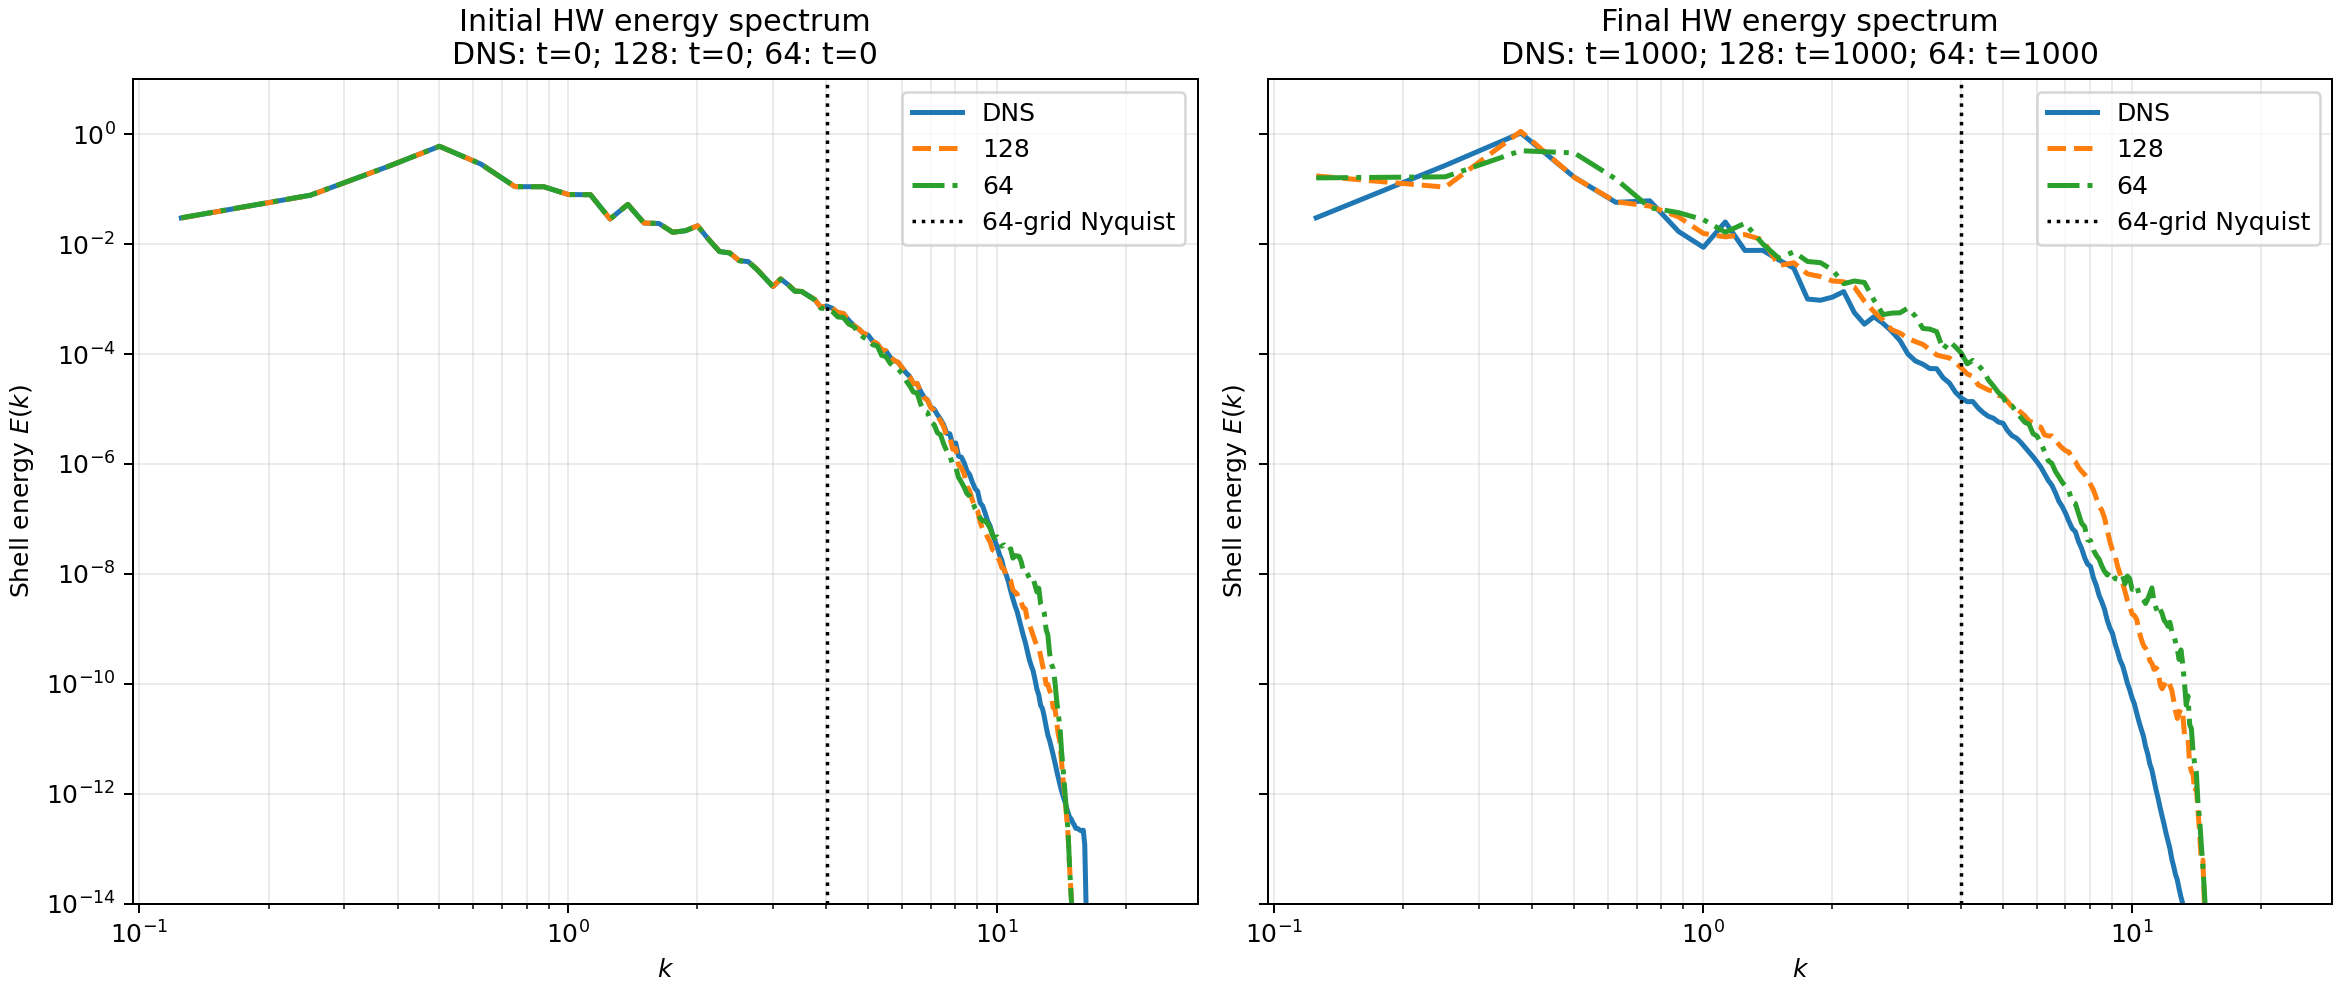
\includegraphics[width=\linewidth,height=0.235\textheight,keepaspectratio]{images/mHW_N256_hw_energy_spectra_initial_final.png}
\caption{\texttt{mHW\_N256}}
\end{subfigure}
\par\smallskip
\begin{subfigure}[t]{0.98\textwidth}
\centering
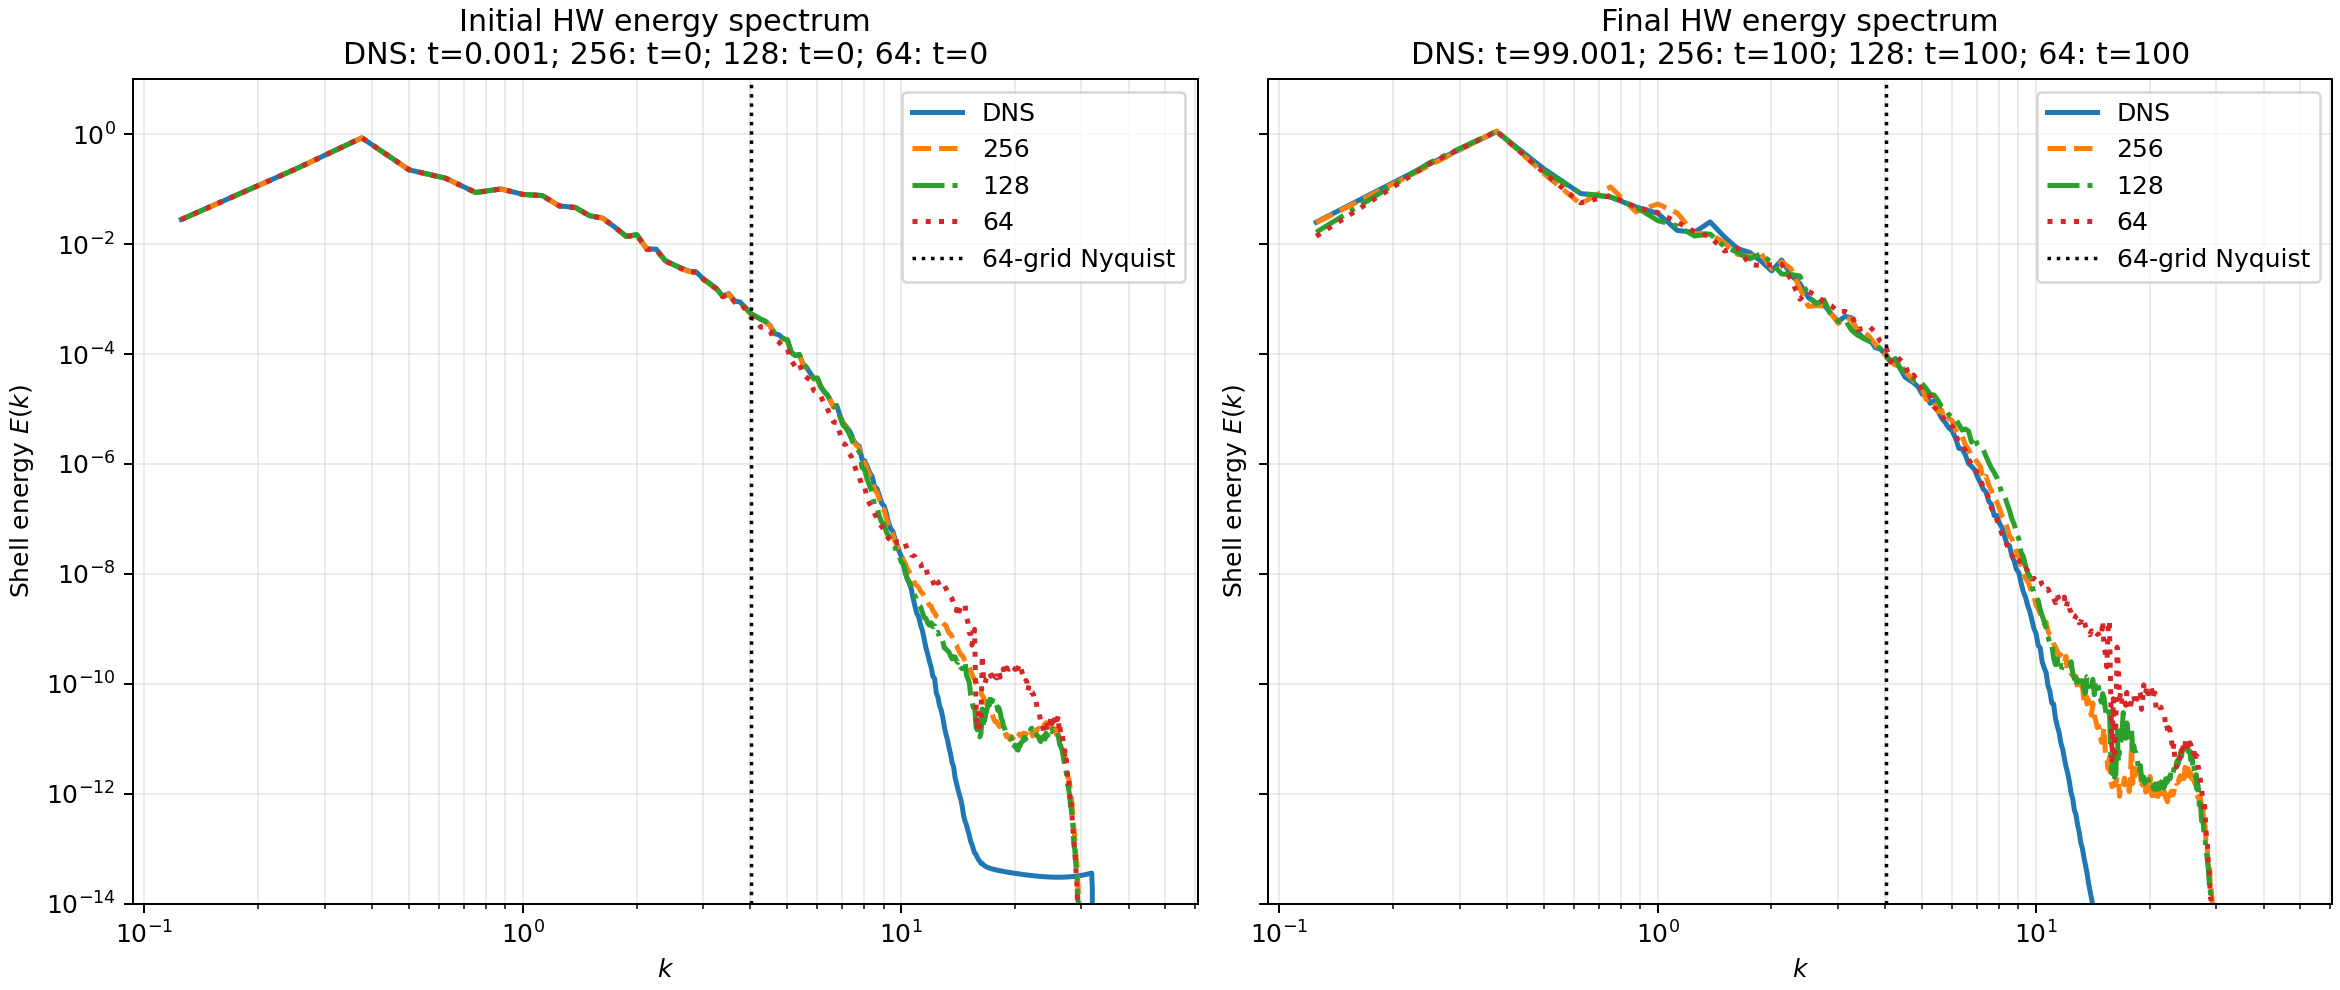
\includegraphics[width=\linewidth,height=0.235\textheight,keepaspectratio]{images/mHW_N512_hw_energy_spectra_initial_final.png}
\caption{\texttt{mHW\_N512}}
\end{subfigure}
\caption{Initial (left) and final (right) shell-summed HW energy spectra for the available cases. Times are those printed in each image: for mHW\_N512 the final DNS snapshot is at $t=99.001$ and the reconstructed snapshots are at $t=100$. The dotted vertical line marks the 64-grid Nyquist wavenumber. HW\_N512 is omitted because its requested endpoint-spectrum image is unavailable.}
\label{fig:spectra}
\end{figure}

\subsection{Probability-density functions}

Figures~\ref{fig:pdf-density}--\ref{fig:pdf-vorticity} compare spatial probability-density functions (PDFs) of density, electrostatic potential and vorticity. The saved channels are $U=n$, $V=\phi$ and $P=\zeta$; the vorticity axes use the equivalent symbol $\omega$. Despite their filenames, these plots contain initial and final snapshot PDFs, not continuously sampled PDF histories or time-averaged distributions.

The initial distributions nearly coincide in all four cases. For HW, the final PDFs retain similar single-peaked shapes, although peak heights and widths differ, especially for the coarsest HW\_N512 reconstruction. In mHW\_N256, larger final discrepancies appear: the DNS density distribution is more sharply peaked, and the potential and vorticity distributions exhibit structures whose locations and amplitudes differ between trajectories. In mHW\_N512, the final distributions remain closer over the shorter interval, including the broad potential distribution and its pronounced peaks. Agreement of these one-point distributions does not establish agreement of spatial organization or density--potential cross-correlations. The linear-scale PDFs do not support a quantitative claim about rare-event tail probabilities.

\begin{figure}[p]
\centering
\begin{subfigure}[t]{0.98\textwidth}
\centering
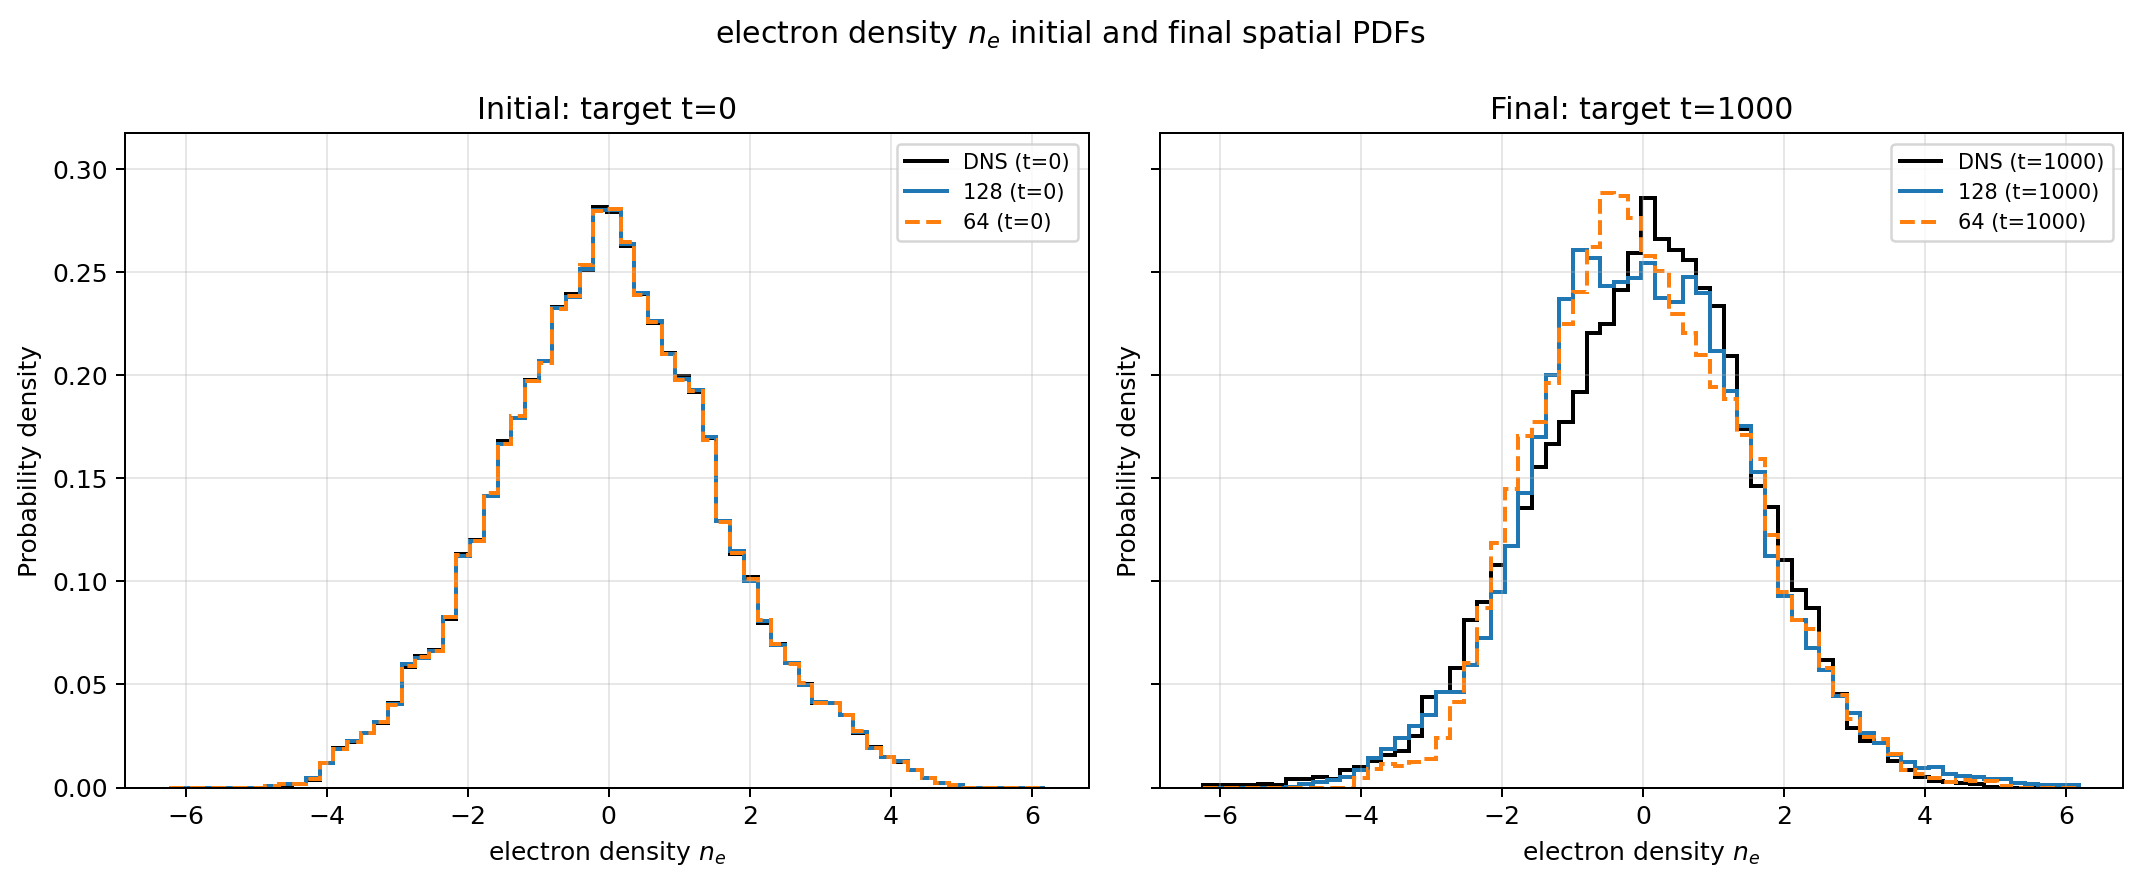
\includegraphics[width=\linewidth,height=0.18\textheight,keepaspectratio]{images/HW_N256_U_pdf_vs_time.png}
\caption{\texttt{HW\_N256}}
\end{subfigure}
\par\smallskip
\begin{subfigure}[t]{0.98\textwidth}
\centering
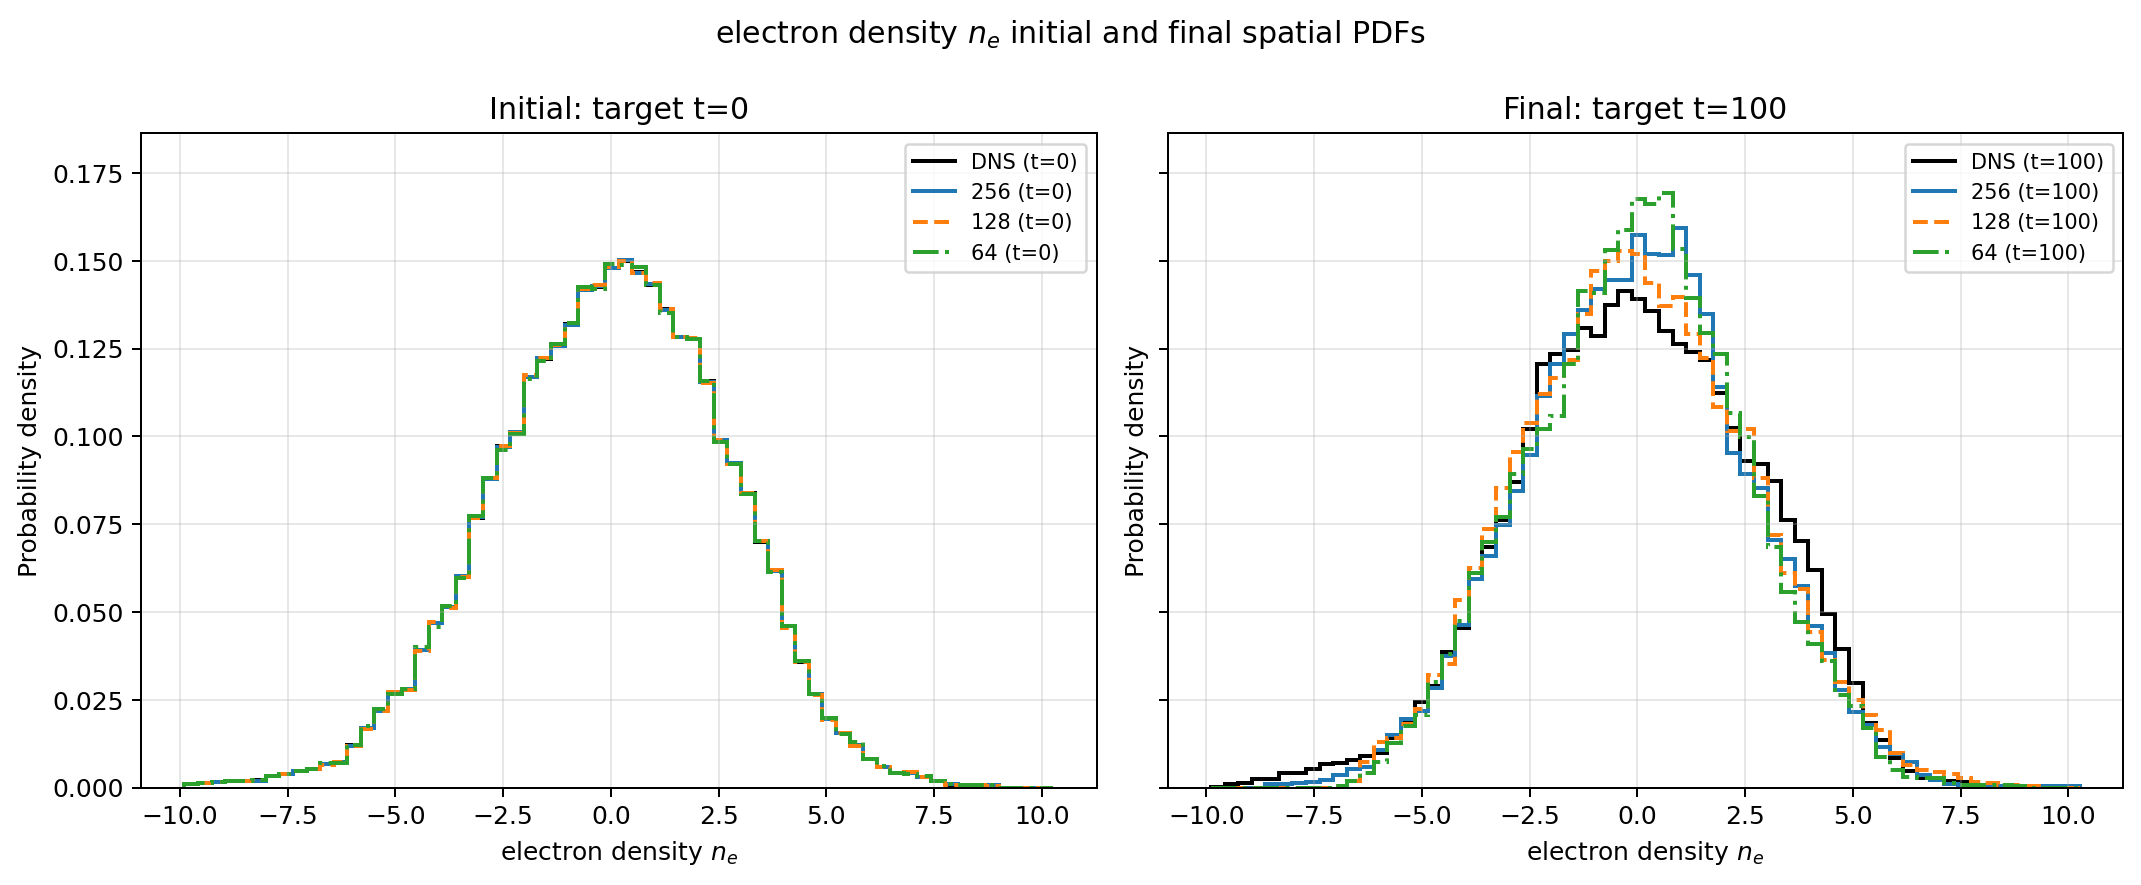
\includegraphics[width=\linewidth,height=0.18\textheight,keepaspectratio]{images/HW_N512_U_pdf_vs_time.png}
\caption{\texttt{HW\_N512}}
\end{subfigure}
\par\smallskip
\begin{subfigure}[t]{0.98\textwidth}
\centering
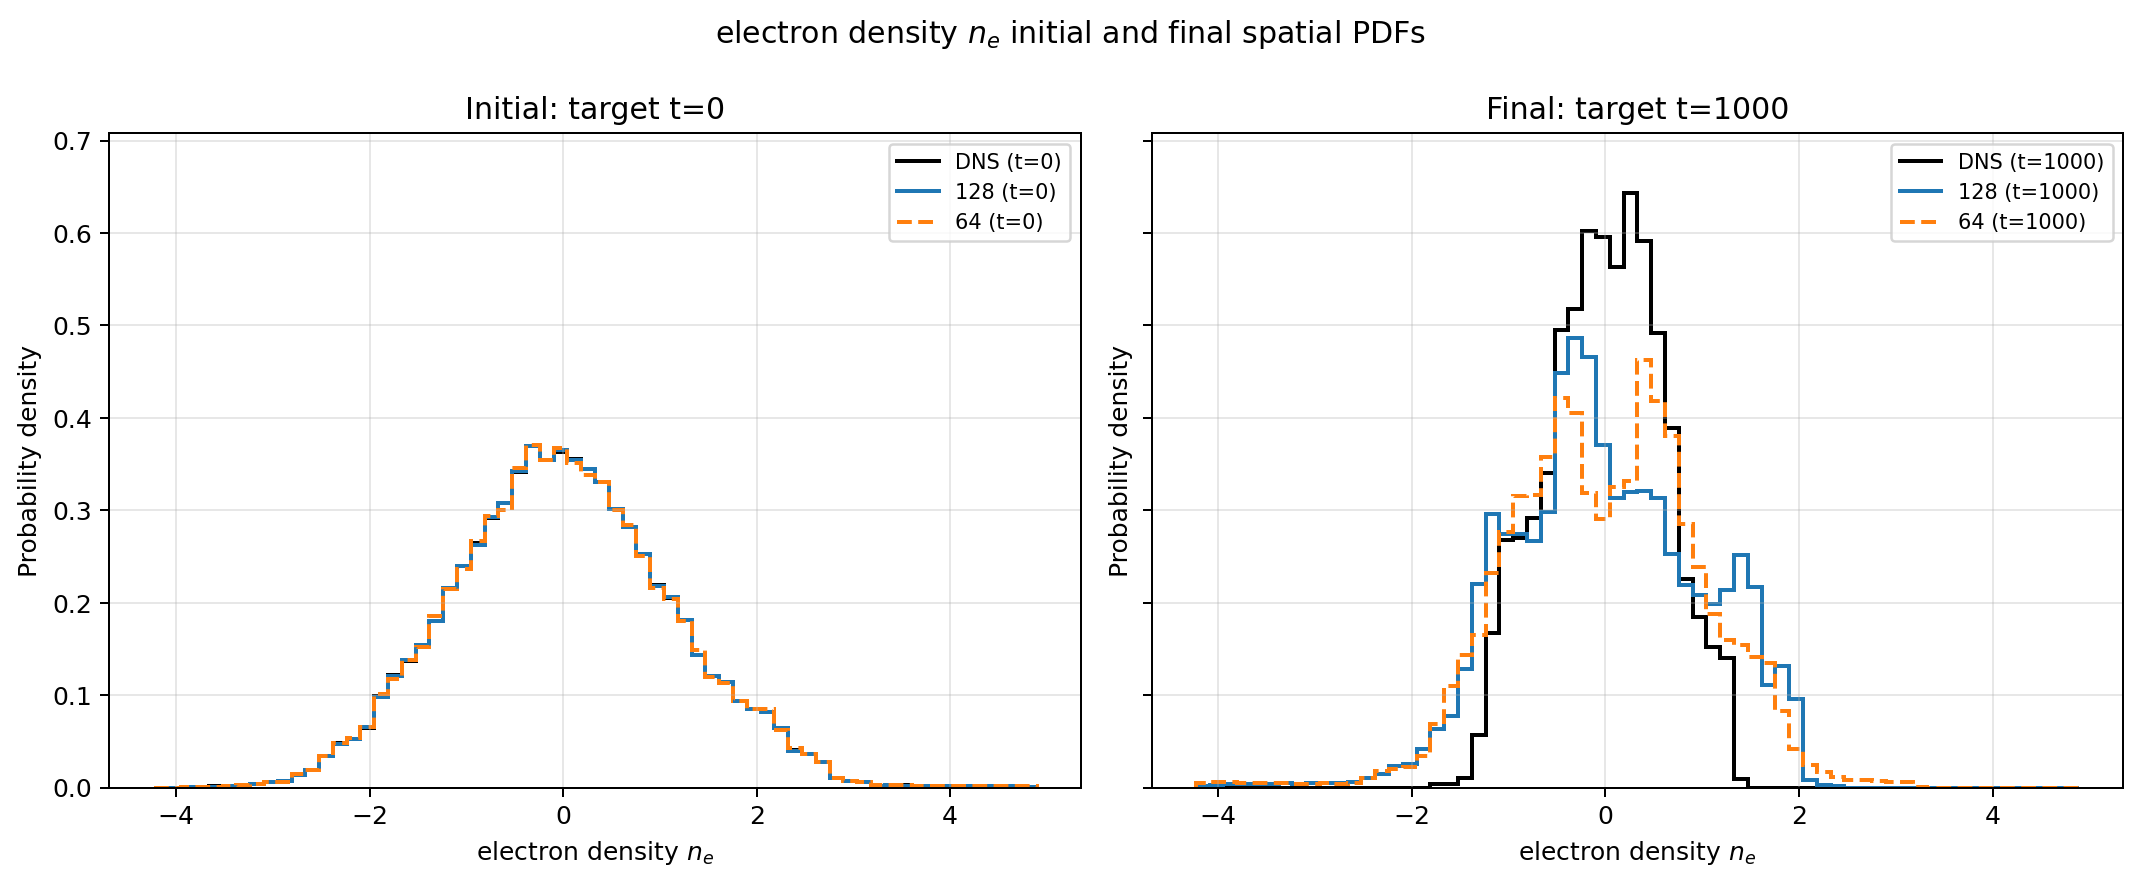
\includegraphics[width=\linewidth,height=0.18\textheight,keepaspectratio]{images/mHW_N256_U_pdf_vs_time.png}
\caption{\texttt{mHW\_N256}}
\end{subfigure}
\par\smallskip
\begin{subfigure}[t]{0.98\textwidth}
\centering
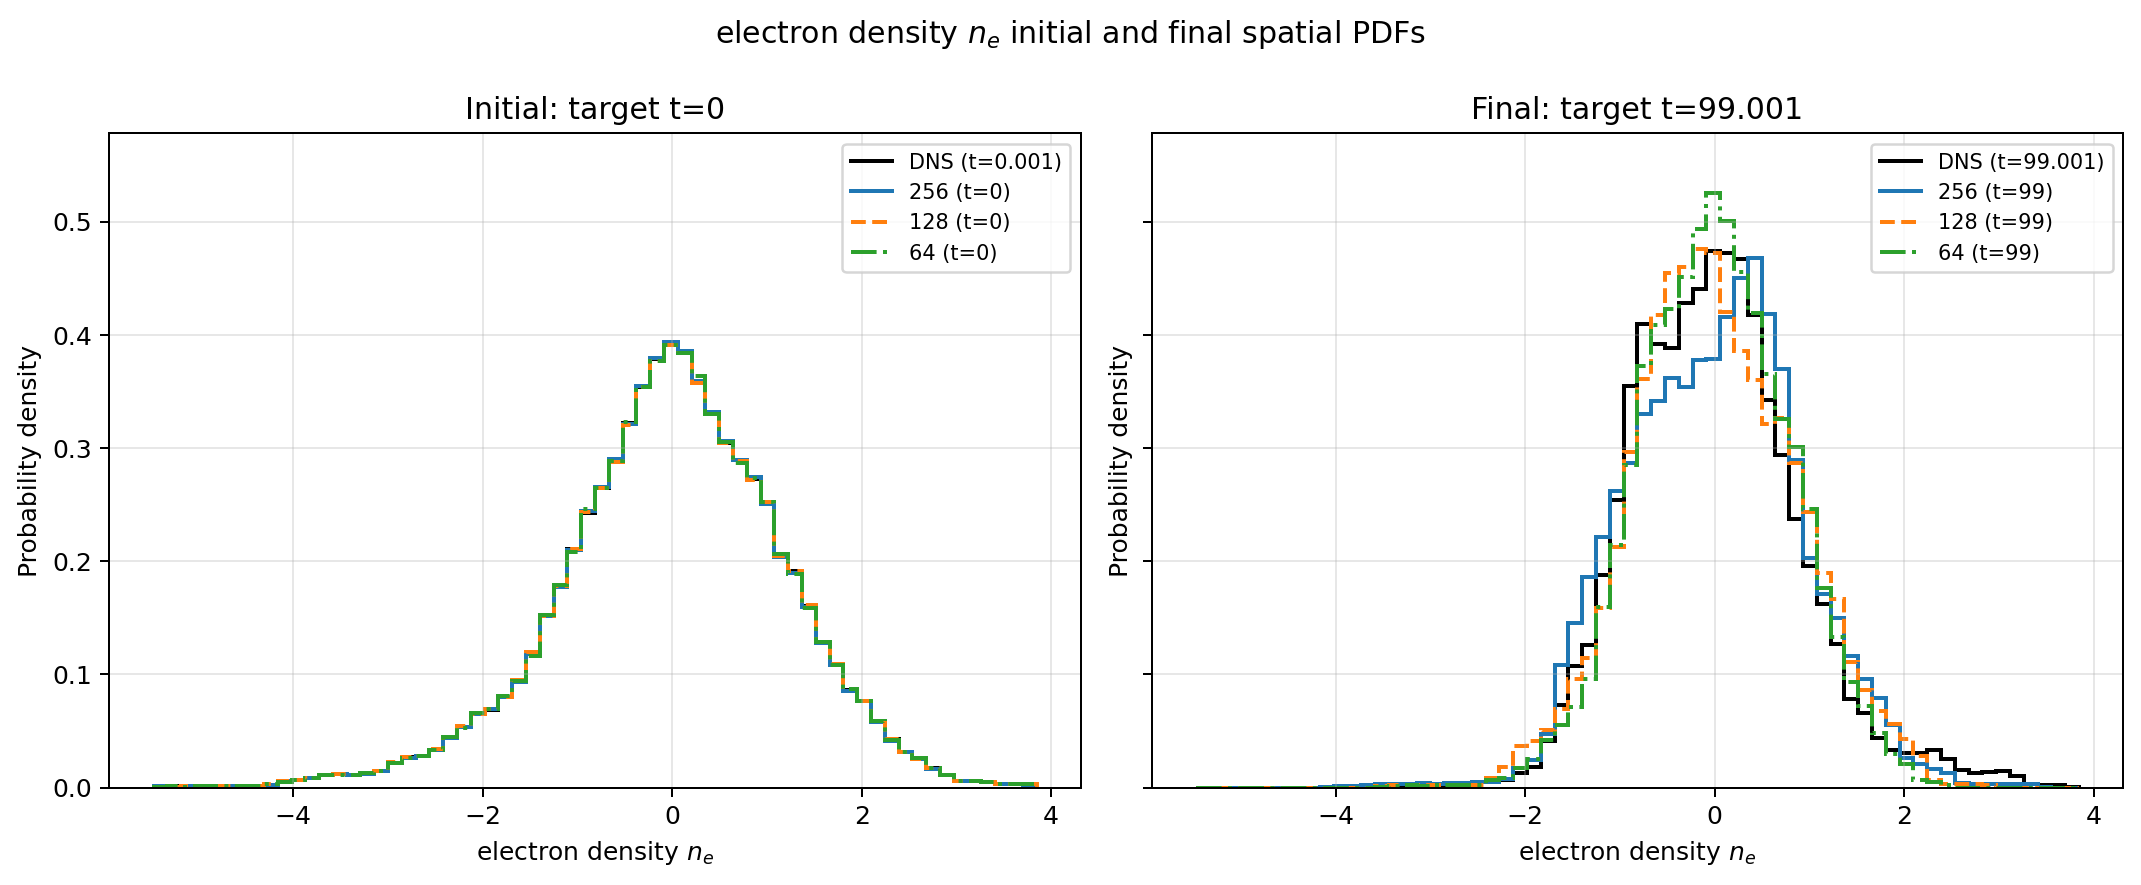
\includegraphics[width=\linewidth,height=0.18\textheight,keepaspectratio]{images/mHW_N512_U_pdf_vs_time.png}
\caption{\texttt{mHW\_N512}}
\end{subfigure}
\caption{Initial (left) and final (right) spatial PDFs of density $n$. The final target is $t=1000$ for the $256^2$ cases and $t=100$ for HW\_N512. For mHW\_N512, the final DNS sample is at $t=99.001$ and reconstruction samples are at $t=99$; actual sample times are printed in the legends.}
\label{fig:pdf-density}
\end{figure}
\begin{figure}[p]
\centering
\begin{subfigure}[t]{0.98\textwidth}
\centering
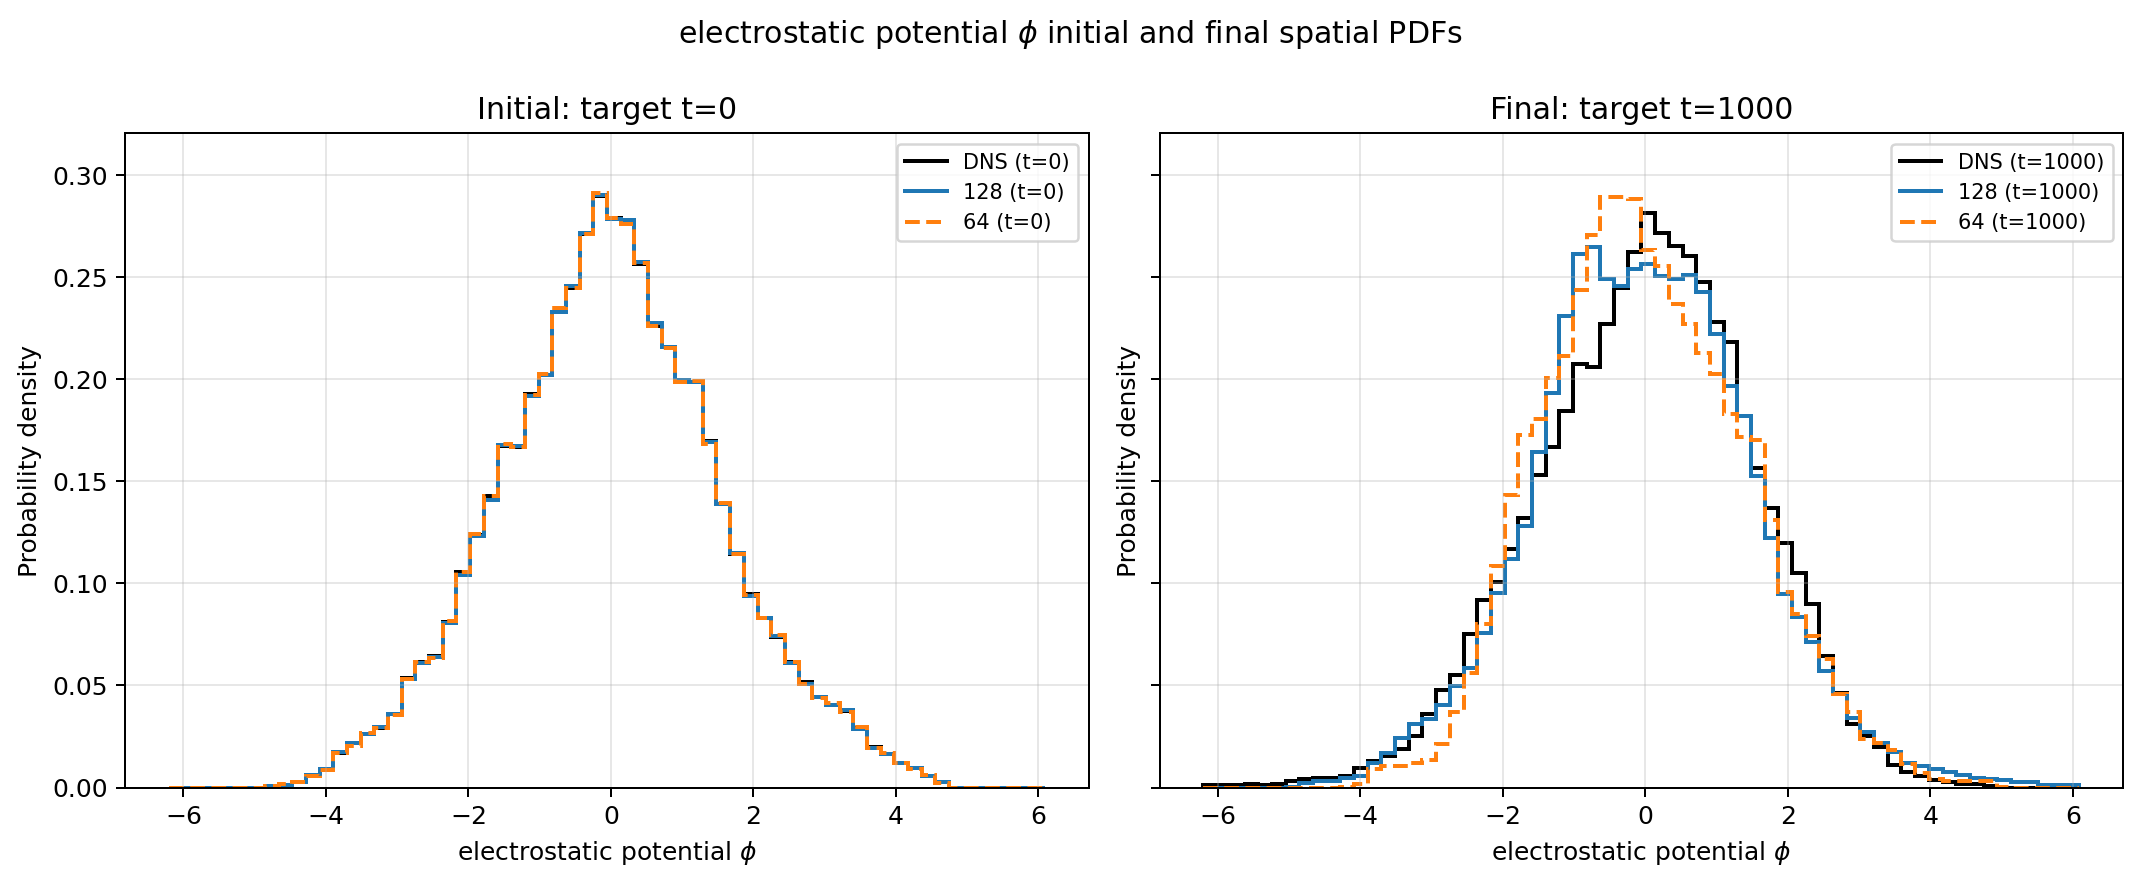
\includegraphics[width=\linewidth,height=0.18\textheight,keepaspectratio]{images/HW_N256_V_pdf_vs_time.png}
\caption{\texttt{HW\_N256}}
\end{subfigure}
\par\smallskip
\begin{subfigure}[t]{0.98\textwidth}
\centering
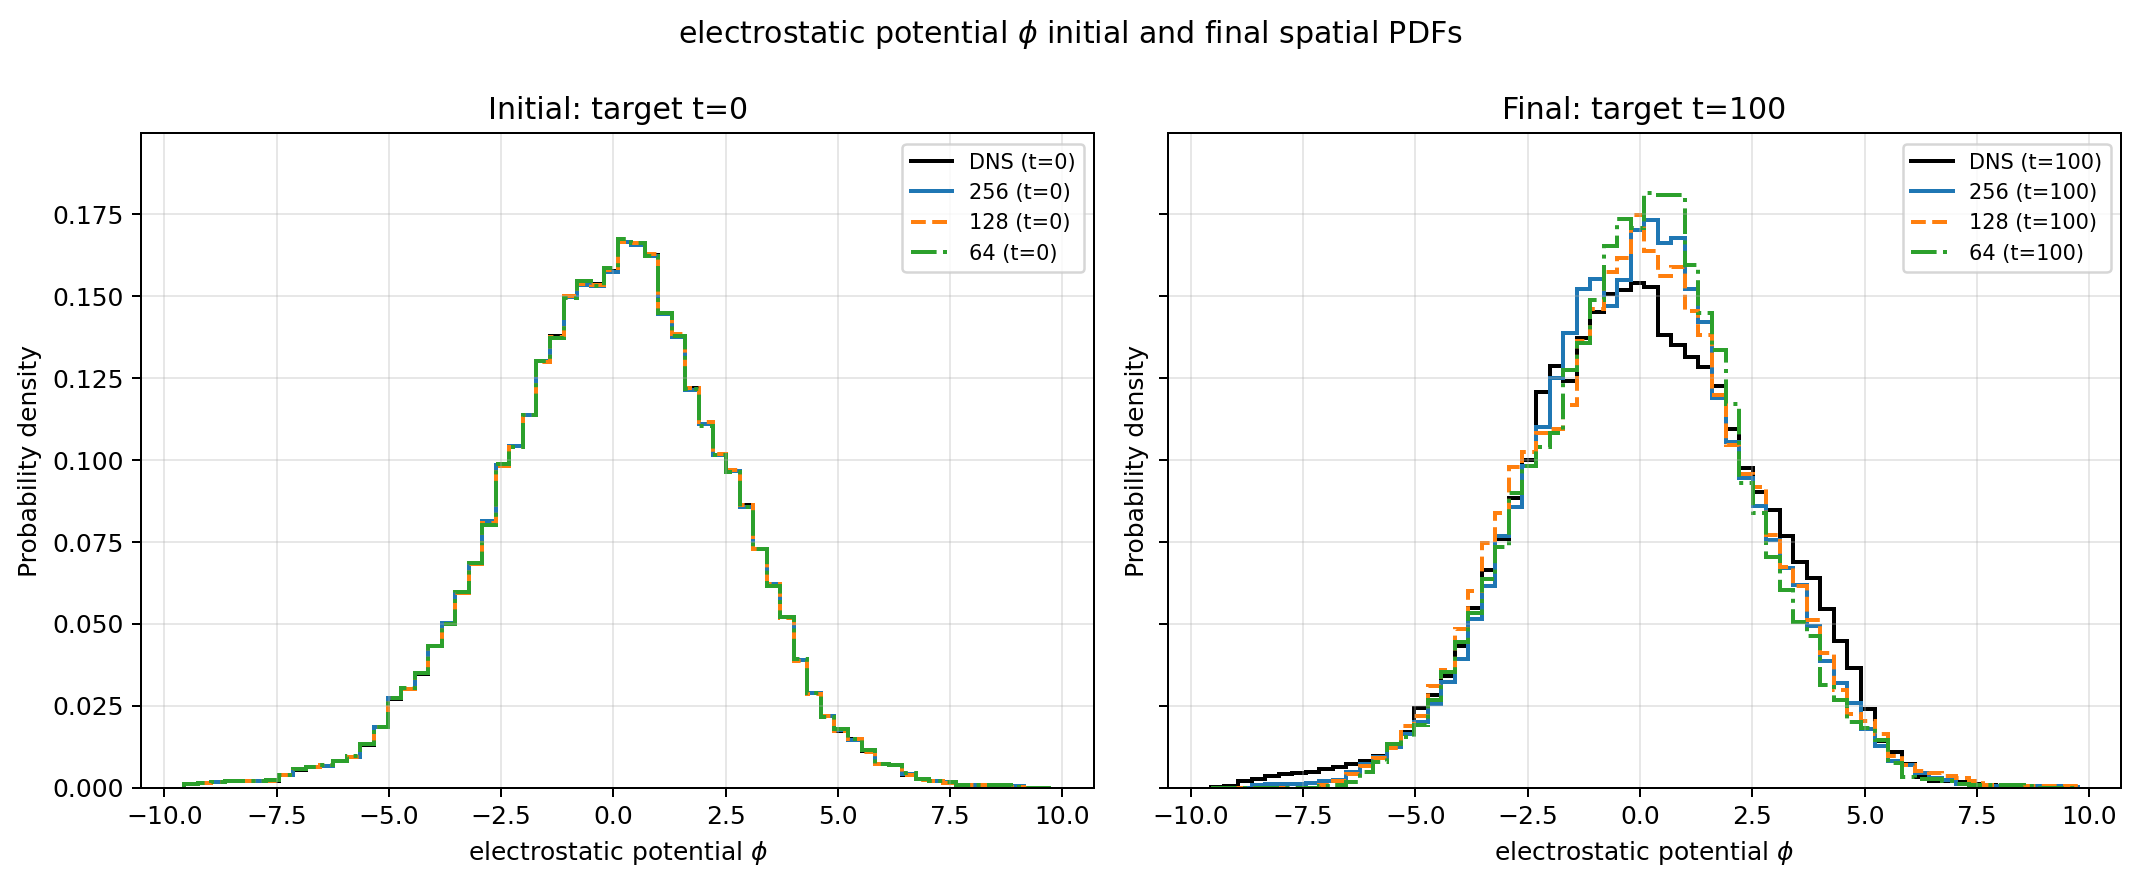
\includegraphics[width=\linewidth,height=0.18\textheight,keepaspectratio]{images/HW_N512_V_pdf_vs_time.png}
\caption{\texttt{HW\_N512}}
\end{subfigure}
\par\smallskip
\begin{subfigure}[t]{0.98\textwidth}
\centering
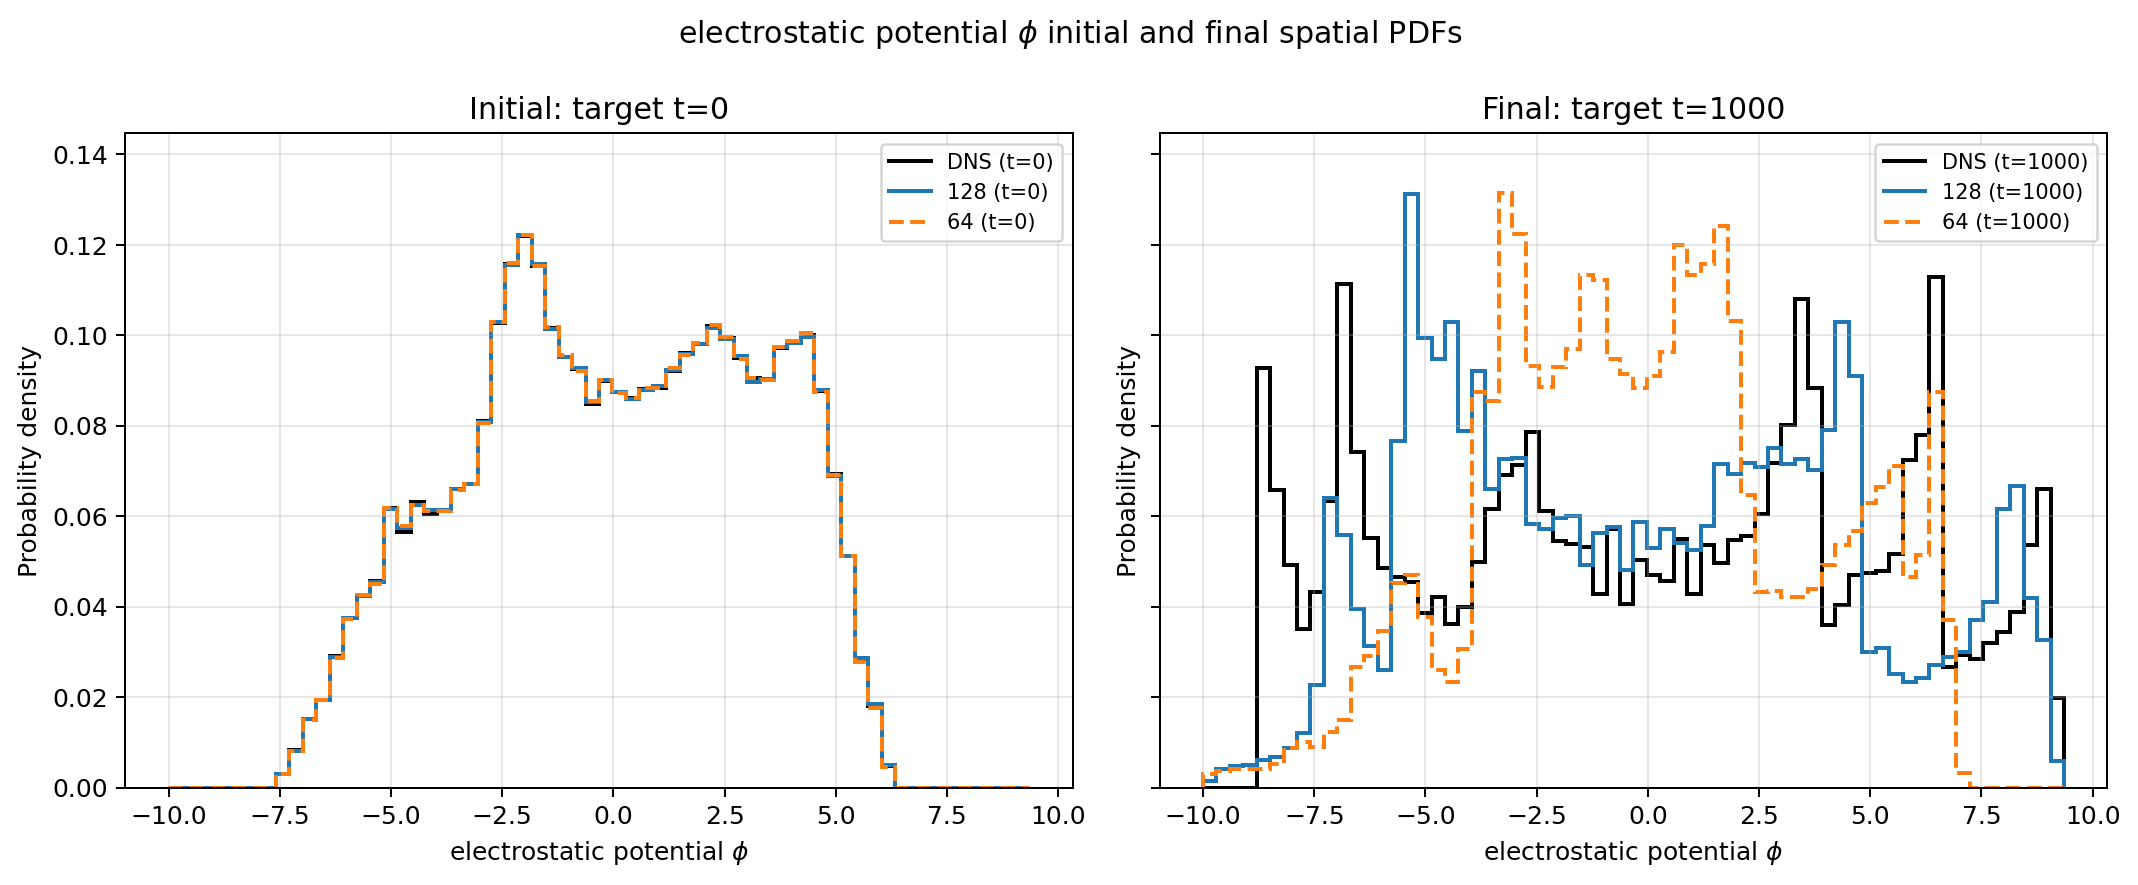
\includegraphics[width=\linewidth,height=0.18\textheight,keepaspectratio]{images/mHW_N256_V_pdf_vs_time.png}
\caption{\texttt{mHW\_N256}}
\end{subfigure}
\par\smallskip
\begin{subfigure}[t]{0.98\textwidth}
\centering
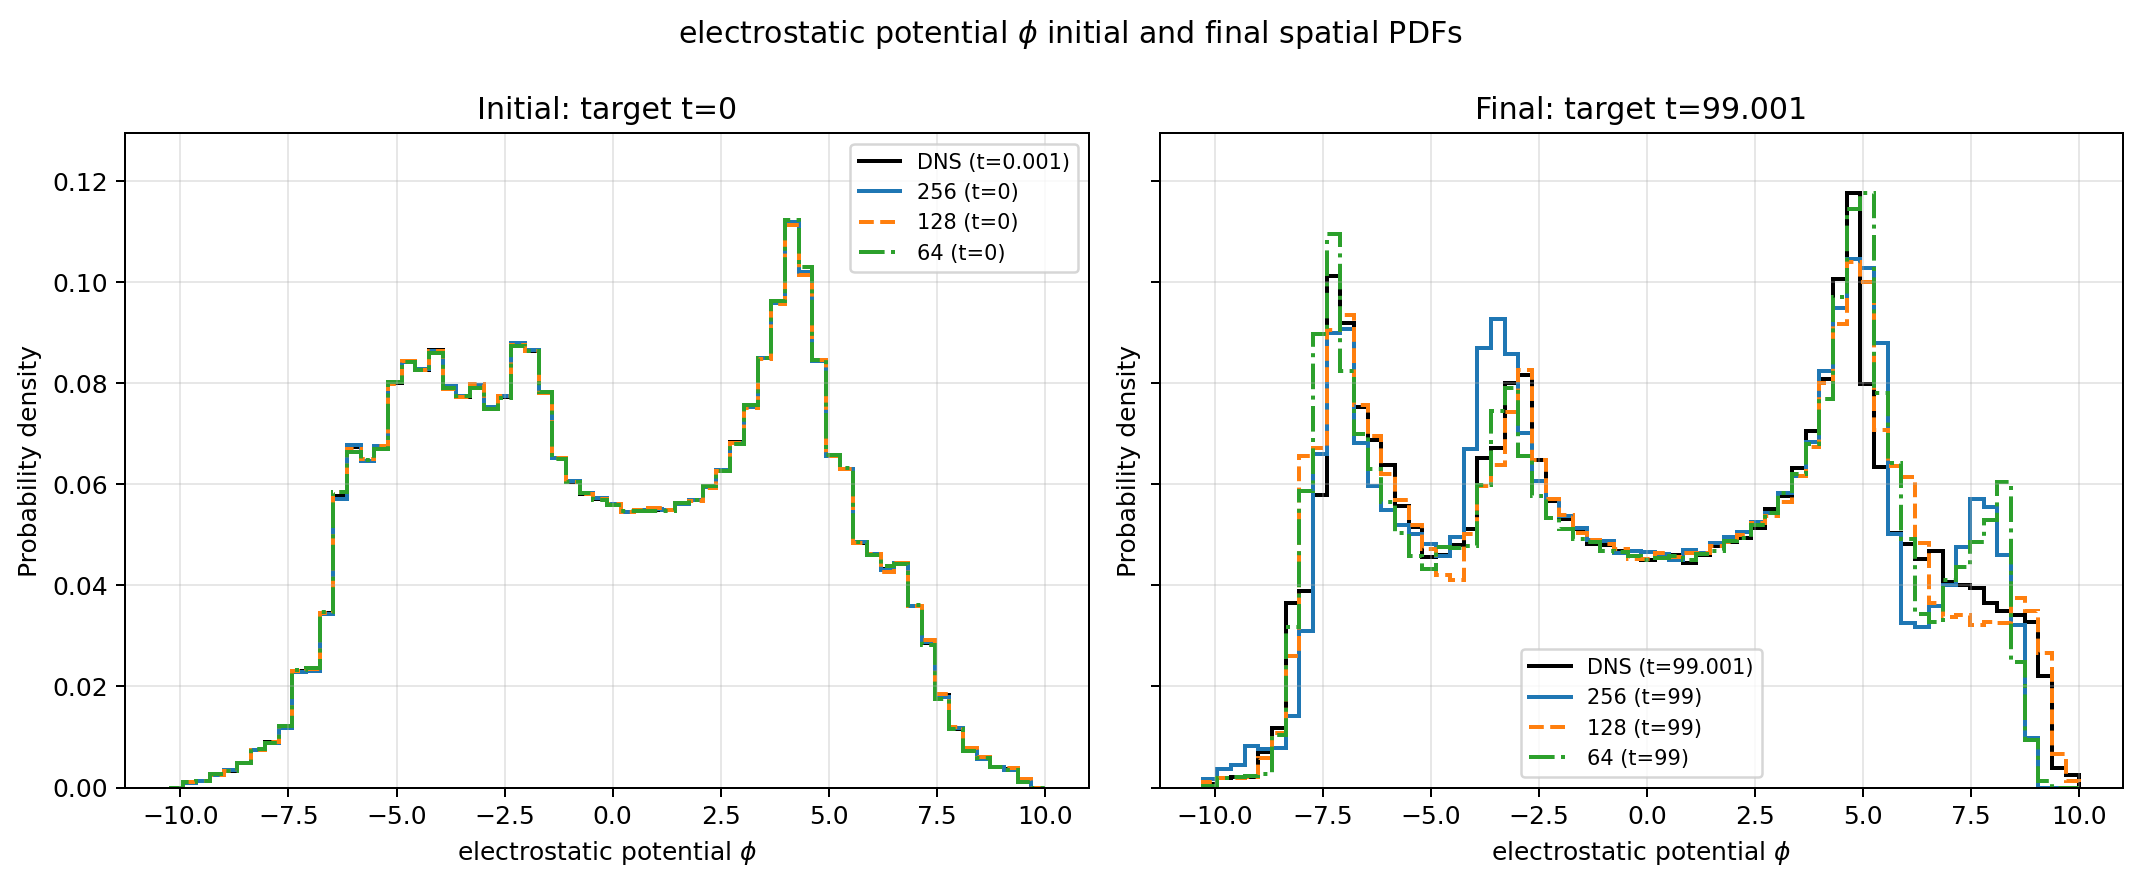
\includegraphics[width=\linewidth,height=0.18\textheight,keepaspectratio]{images/mHW_N512_V_pdf_vs_time.png}
\caption{\texttt{mHW\_N512}}
\end{subfigure}
\caption{Initial (left) and final (right) spatial PDFs of electrostatic potential $\phi$. The final target is $t=1000$ for the $256^2$ cases and $t=100$ for HW\_N512. For mHW\_N512, the final DNS sample is at $t=99.001$ and reconstruction samples are at $t=99$; actual sample times are printed in the legends.}
\label{fig:pdf-potential}
\end{figure}
\begin{figure}[p]
\centering
\begin{subfigure}[t]{0.98\textwidth}
\centering
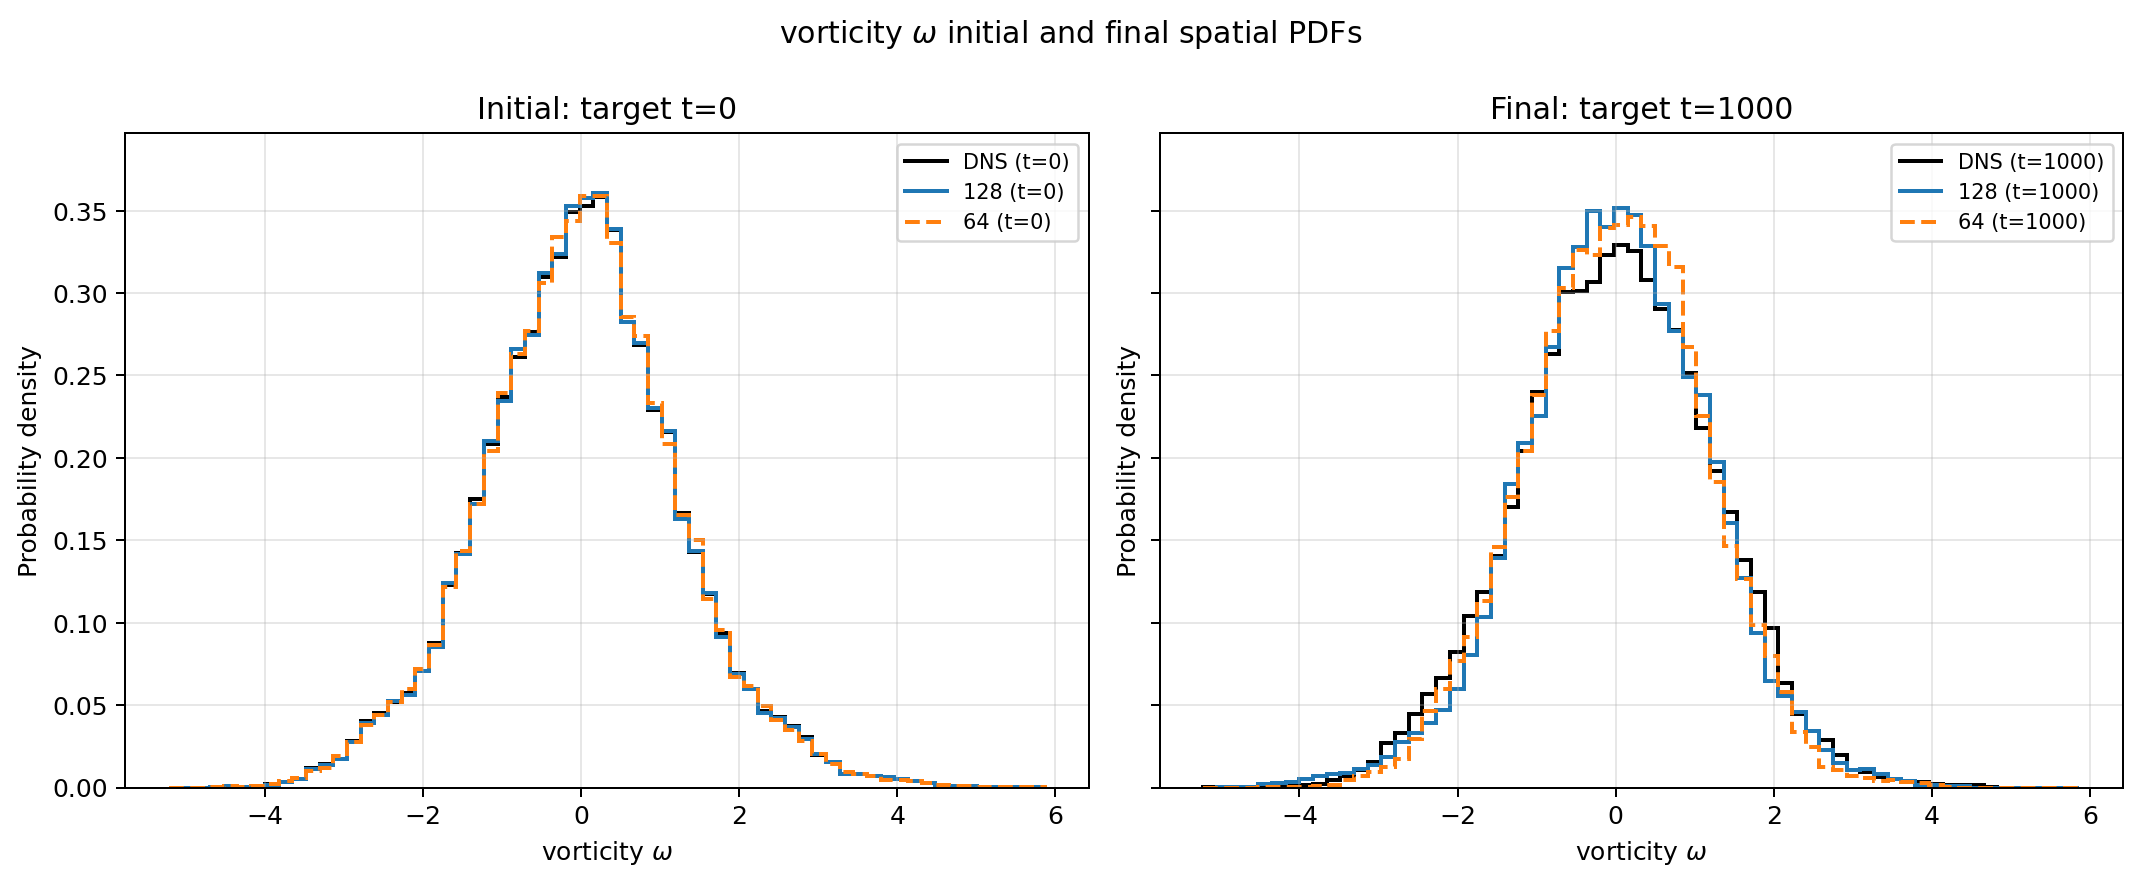
\includegraphics[width=\linewidth,height=0.18\textheight,keepaspectratio]{images/HW_N256_P_pdf_vs_time.png}
\caption{\texttt{HW\_N256}}
\end{subfigure}
\par\smallskip
\begin{subfigure}[t]{0.98\textwidth}
\centering
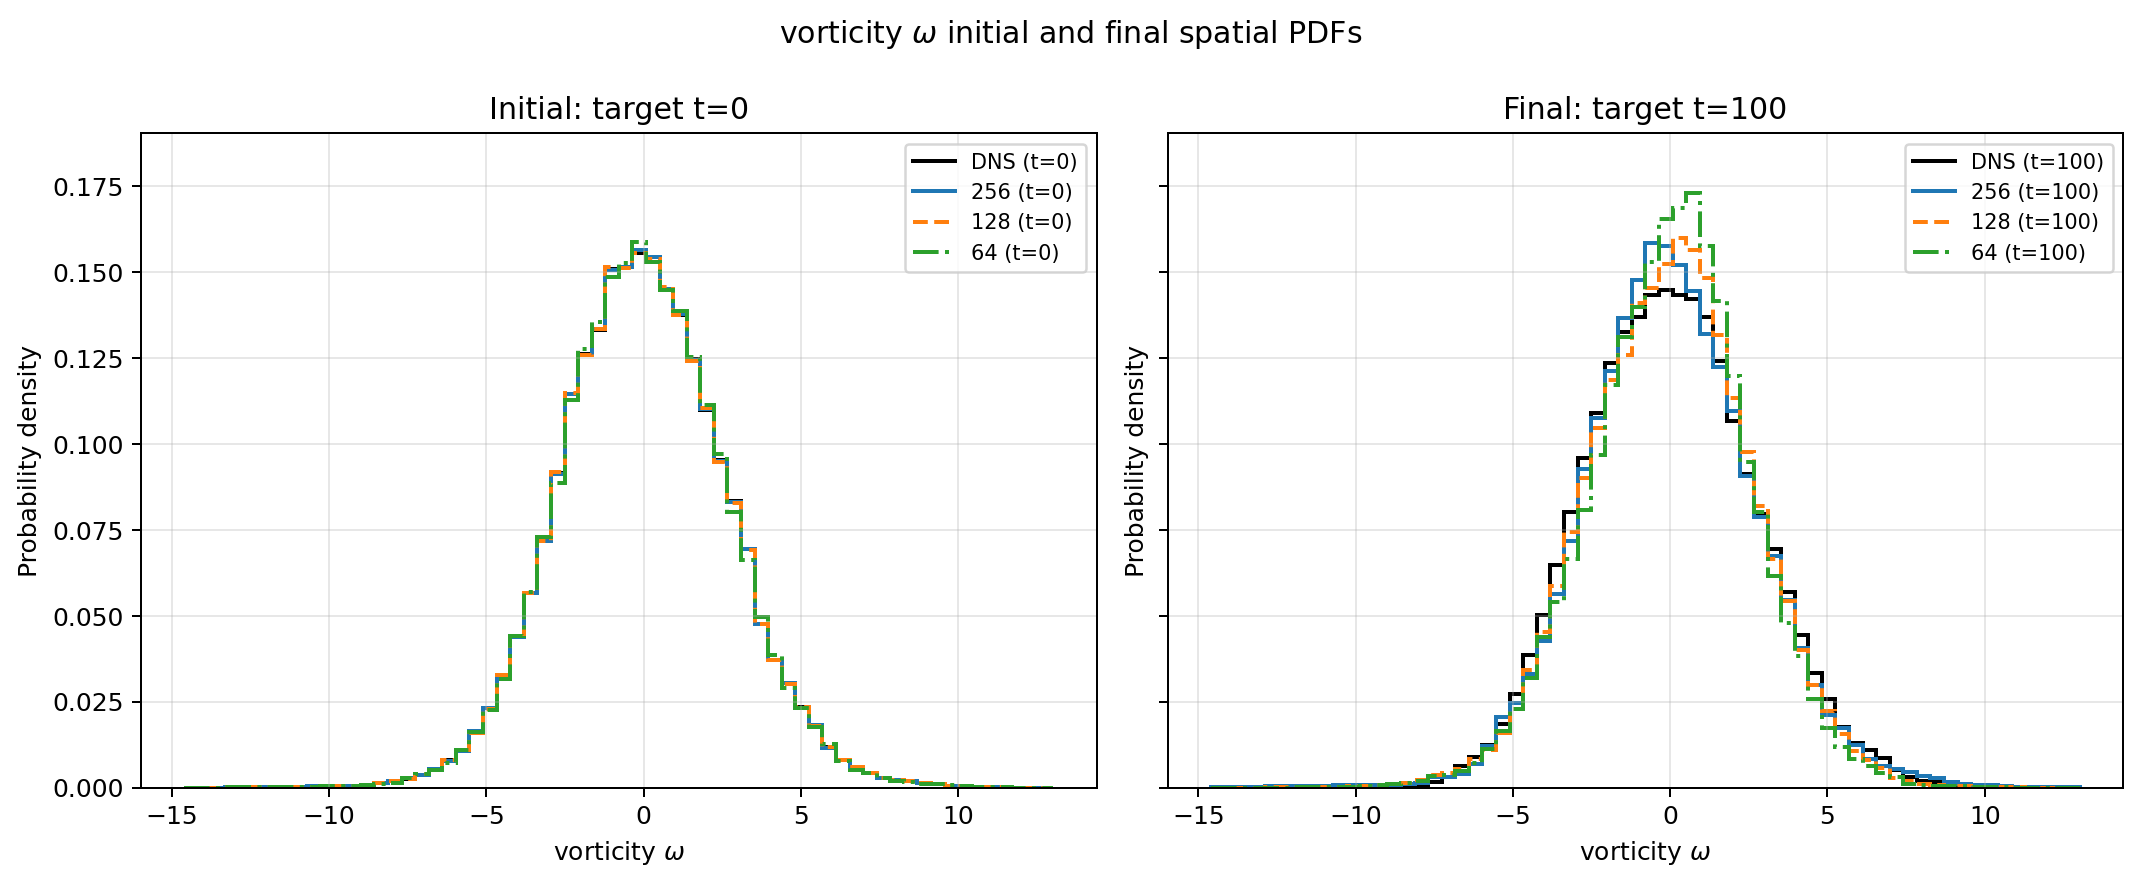
\includegraphics[width=\linewidth,height=0.18\textheight,keepaspectratio]{images/HW_N512_P_pdf_vs_time.png}
\caption{\texttt{HW\_N512}}
\end{subfigure}
\par\smallskip
\begin{subfigure}[t]{0.98\textwidth}
\centering
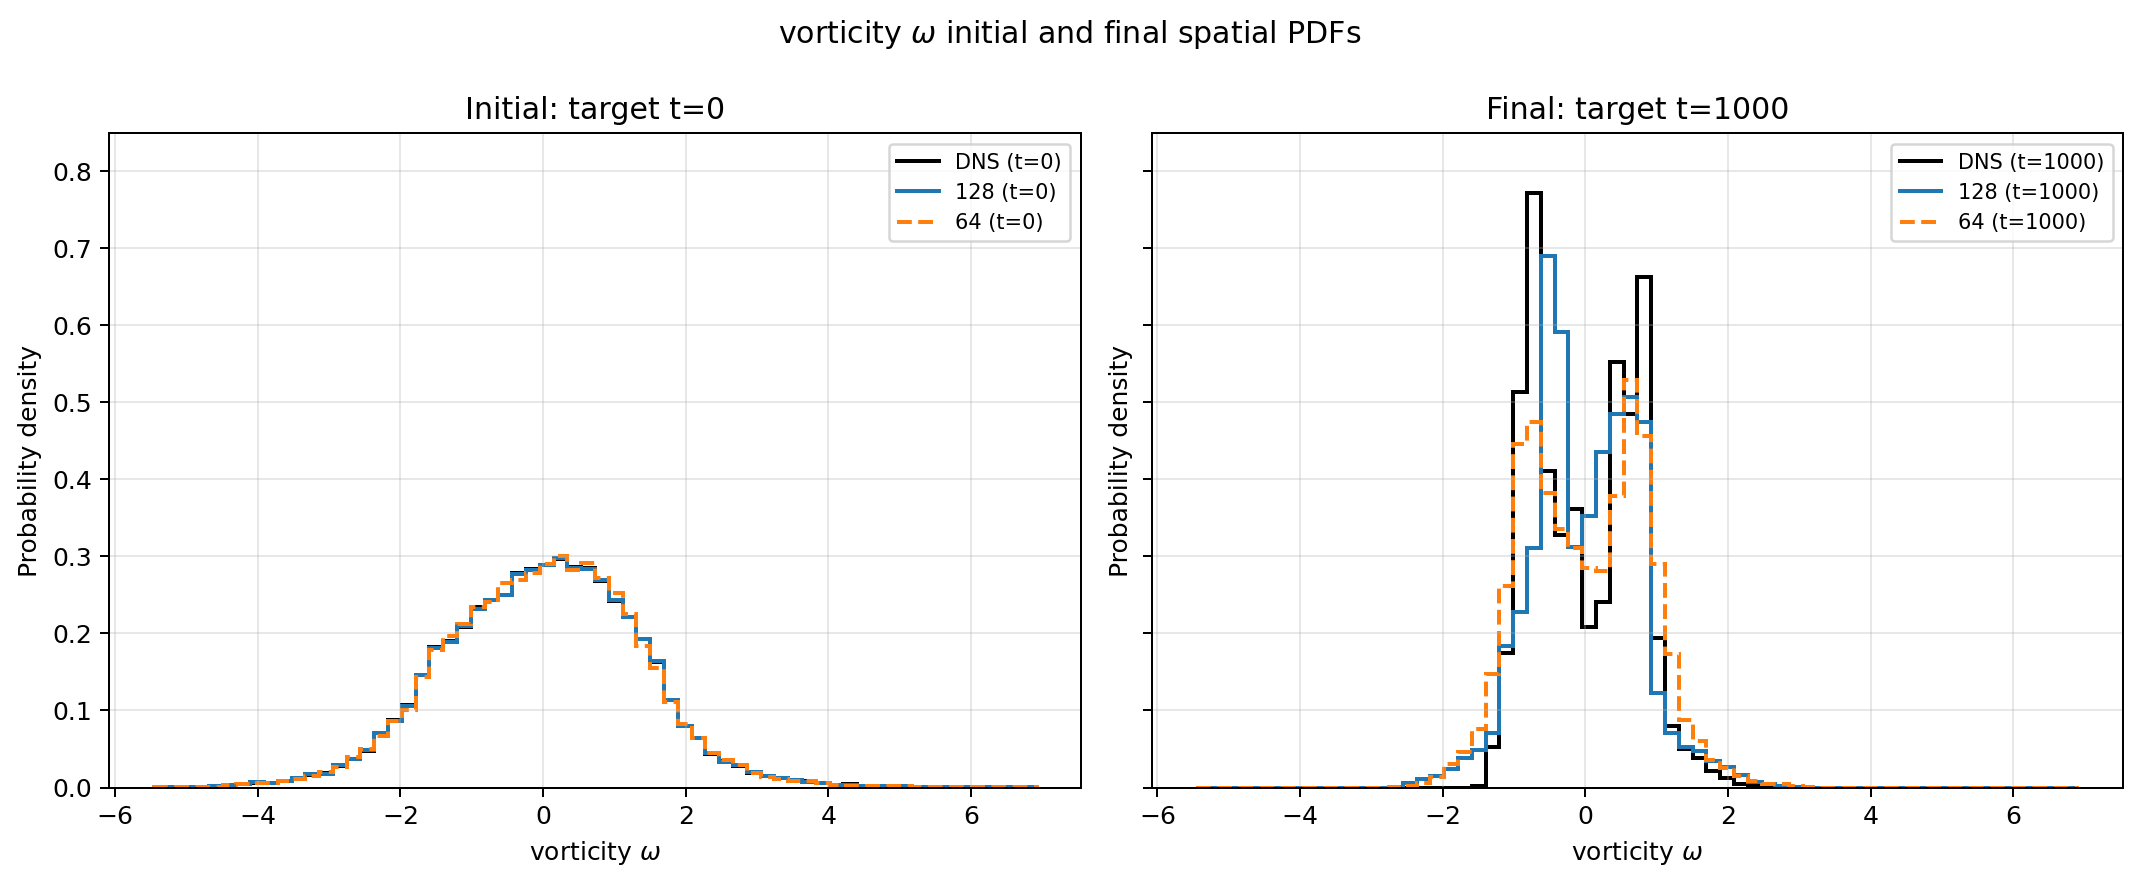
\includegraphics[width=\linewidth,height=0.18\textheight,keepaspectratio]{images/mHW_N256_P_pdf_vs_time.png}
\caption{\texttt{mHW\_N256}}
\end{subfigure}
\par\smallskip
\begin{subfigure}[t]{0.98\textwidth}
\centering
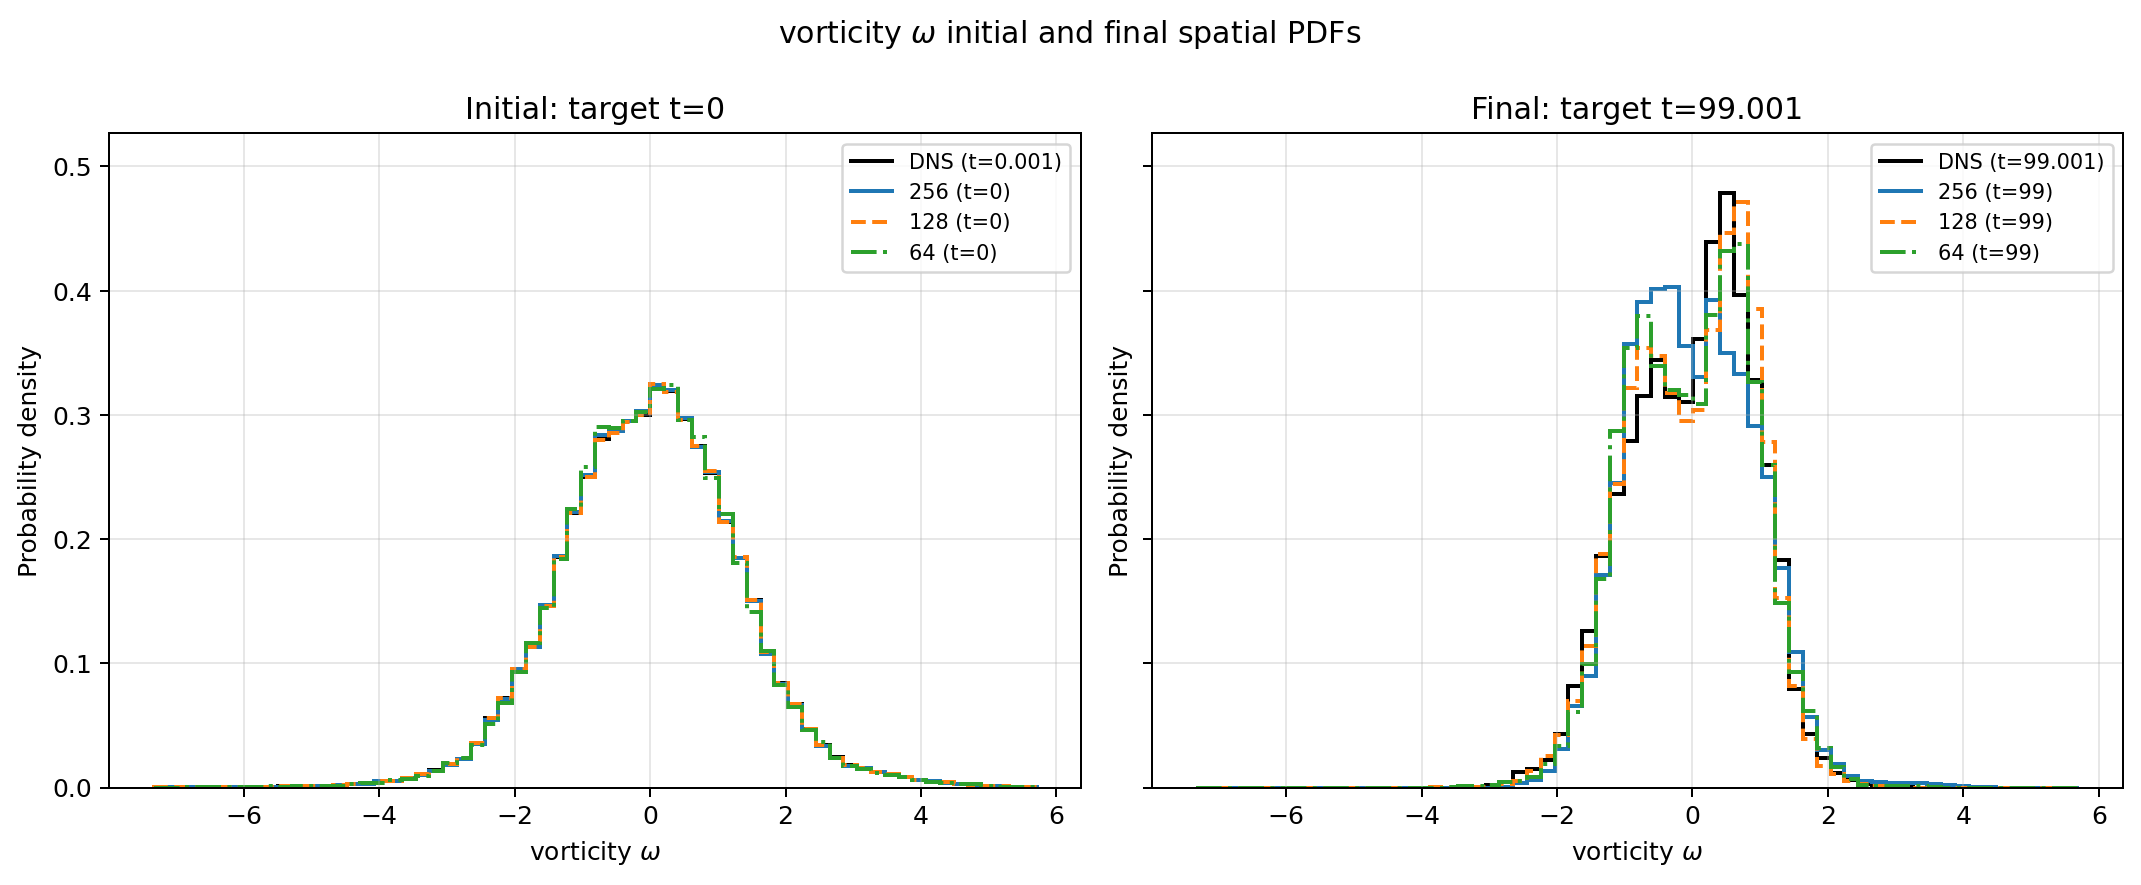
\includegraphics[width=\linewidth,height=0.18\textheight,keepaspectratio]{images/mHW_N512_P_pdf_vs_time.png}
\caption{\texttt{mHW\_N512}}
\end{subfigure}
\caption{Initial (left) and final (right) spatial PDFs of vorticity $\zeta$ (labelled $\omega$ in the images). The final target is $t=1000$ for the $256^2$ cases and $t=100$ for HW\_N512. For mHW\_N512, the final DNS sample is at $t=99.001$ and reconstruction samples are at $t=99$; actual sample times are printed in the legends.}
\label{fig:pdf-vorticity}
\end{figure}

\subsection{Transport diagnostics}

The archived particle-flux histories use the non-zonal density $n'=n-\langle n\rangle_y$ and the velocities
\begin{equation}
 v_x=-\partial_y\phi,\qquad v_y=\partial_x\phi.
\end{equation}
The plotted quantities are domain-averaged turbulent fluxes,
\begin{equation}
 \overline\Gamma_x=-\langle n'\partial_y\phi\rangle_{x,y},\qquad
 \overline\Gamma_y=\langle n'\partial_x\phi\rangle_{x,y}.
\end{equation}
Here the prime denotes removal of the poloidal mean, distinct from the LES spatial filter denoted by a tilde elsewhere. The poloidal flux therefore excludes transport by the zonal density component.

Figure~\ref{fig:particle-flux} shows positive radial flux throughout the plotted intervals. In the HW cases, the reconstructions preserve its overall scale, but the coarsest solution generally underpredicts it and the temporal fluctuations differ from DNS. For mHW\_N256, the initial radial-flux decay is reproduced, while the subsequent burst is delayed, in parallel with the energy and enstrophy transients. The mHW\_N512 radial-flux decay is followed more closely over the available interval. Poloidal flux is smaller and changes sign; its detailed timing is less consistently reproduced, particularly after the initial transient. These results support qualitative transport agreement in some intervals, but not a uniform error bound or a quantified temporal correlation.

\begin{figure}[p]
\centering
\begin{subfigure}[t]{0.48\textwidth}
\centering
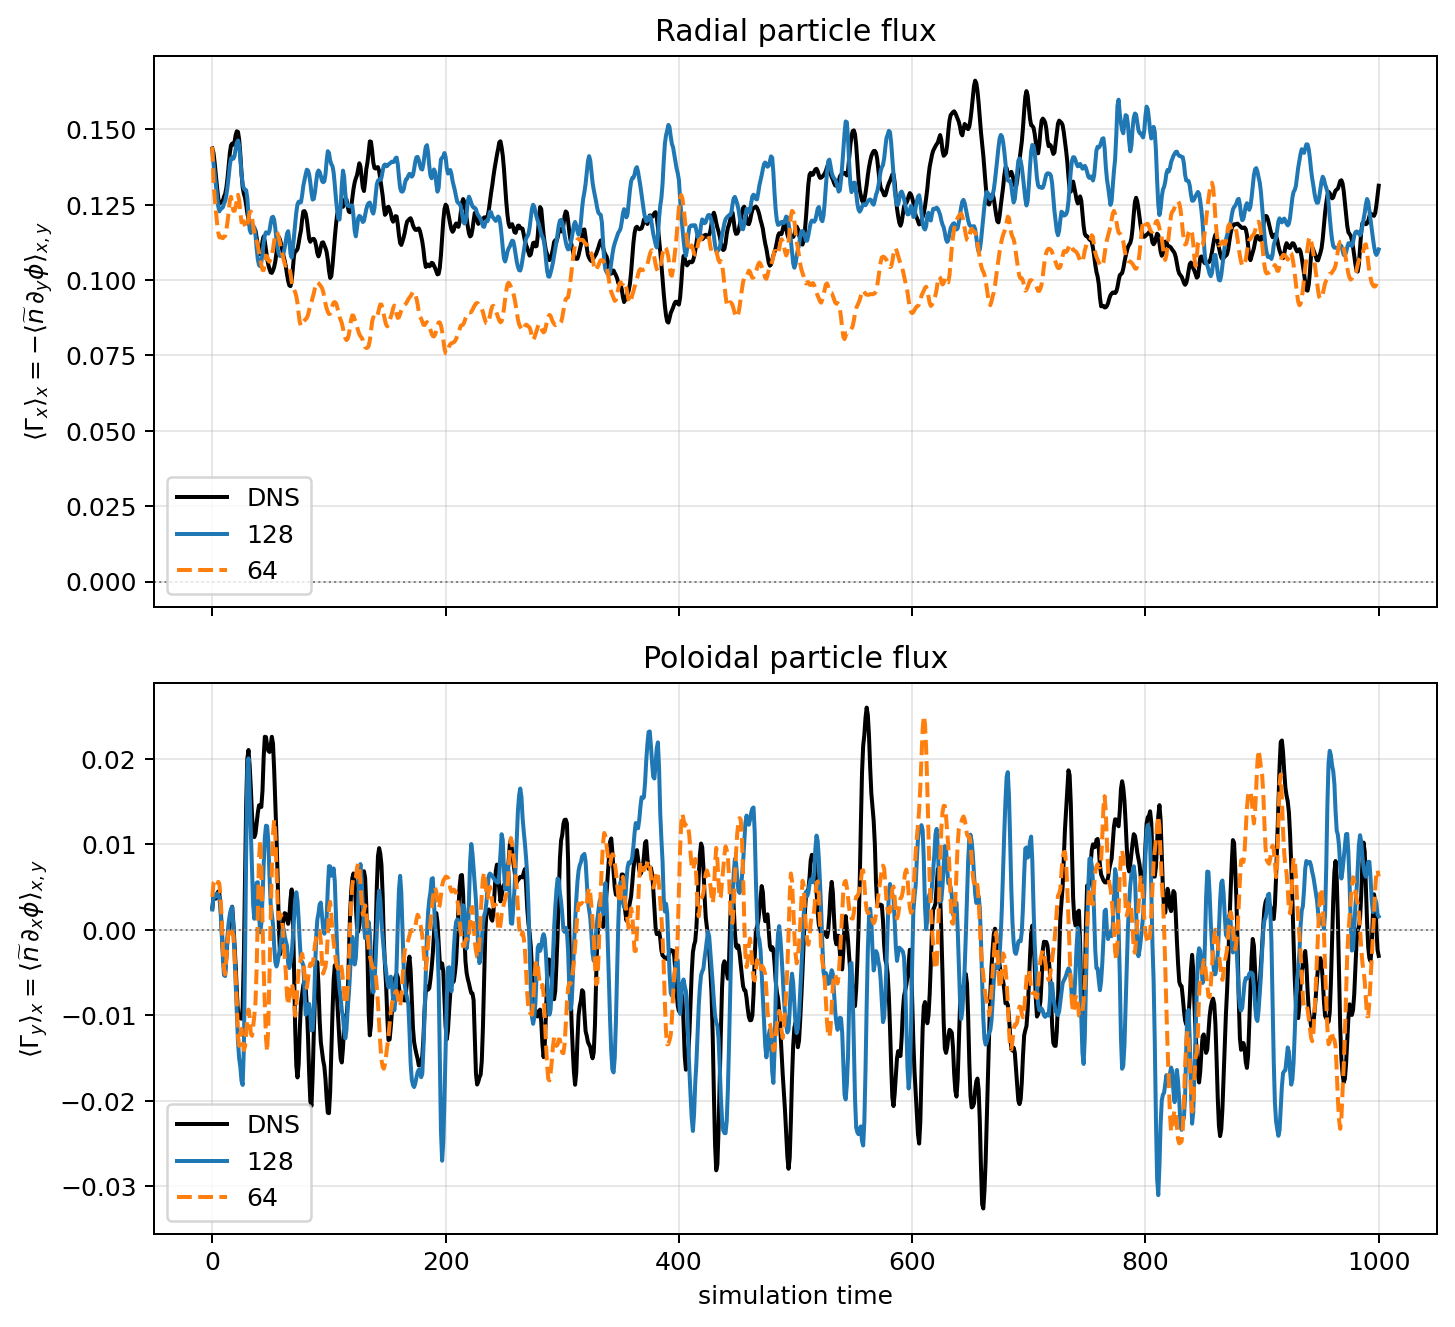
\includegraphics[width=\linewidth]{images/HW_N256_particle_flux_vs_time.png}
\caption{\texttt{HW\_N256}}
\end{subfigure}
\hfill
\begin{subfigure}[t]{0.48\textwidth}
\centering
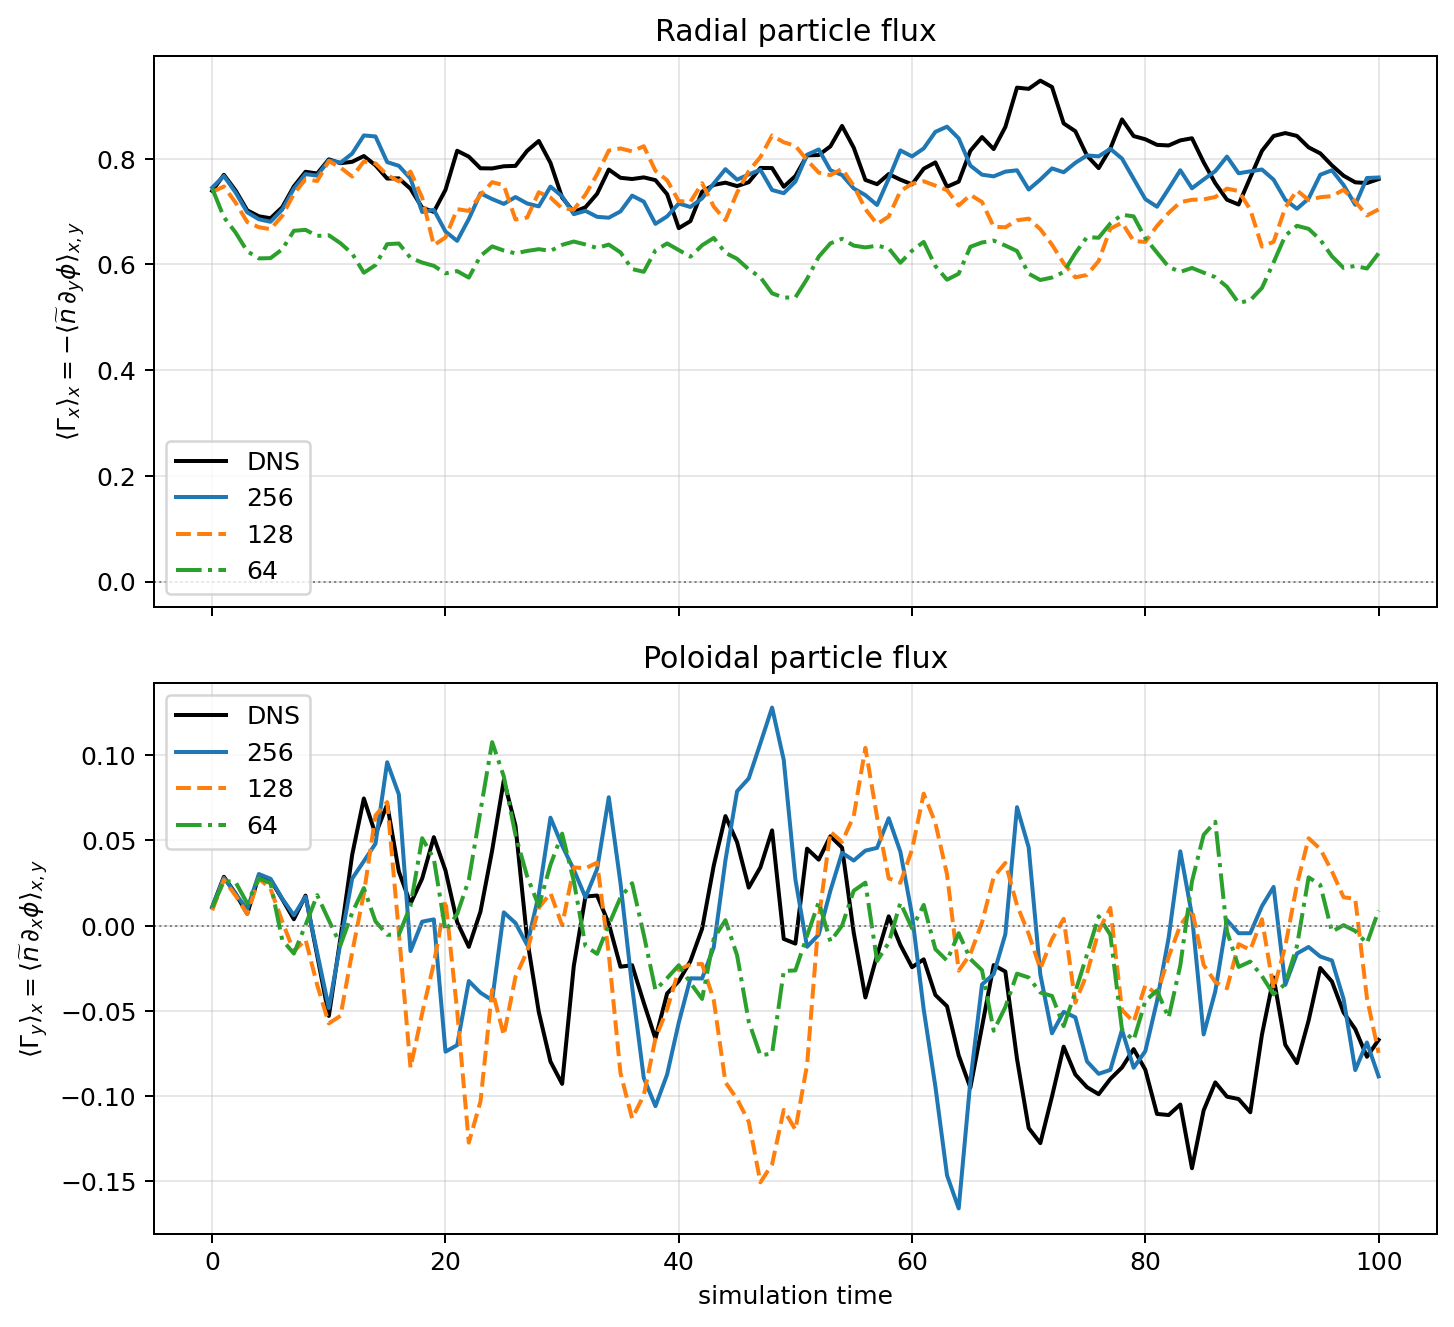
\includegraphics[width=\linewidth]{images/HW_N512_particle_flux_vs_time.png}
\caption{\texttt{HW\_N512}}
\end{subfigure}
\par\smallskip
\begin{subfigure}[t]{0.48\textwidth}
\centering
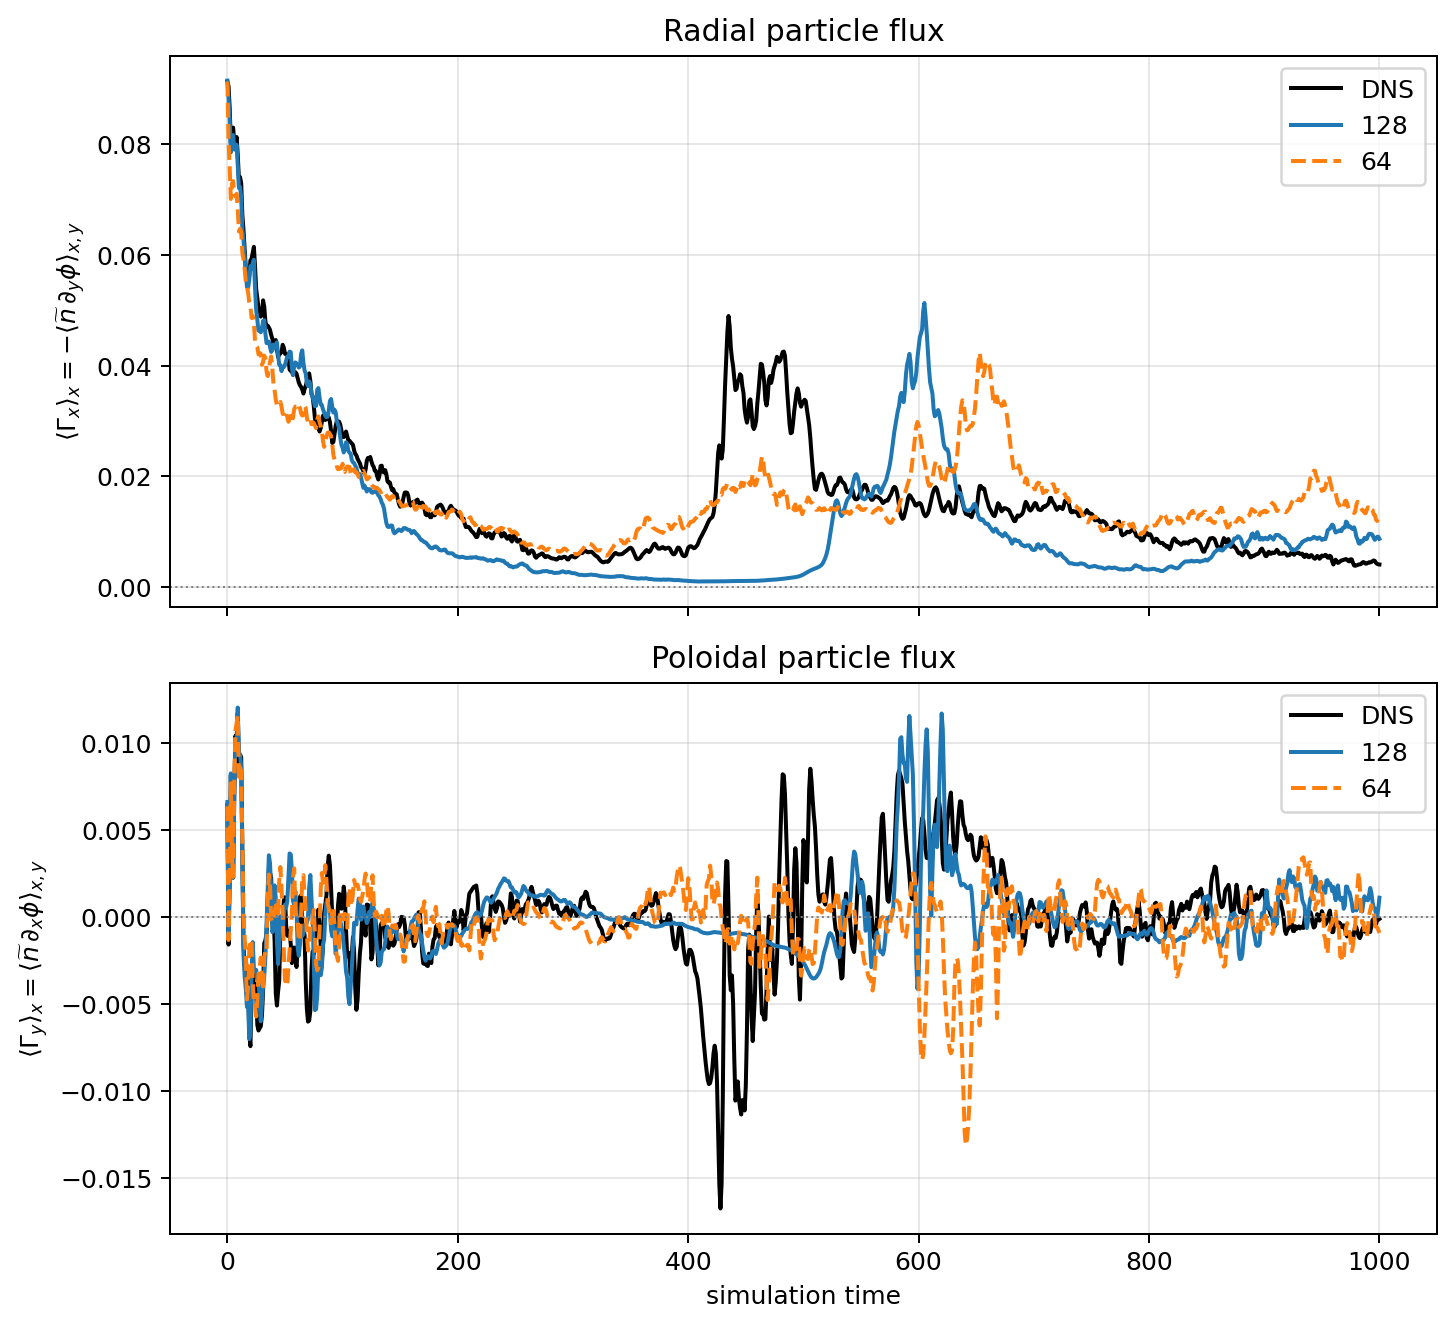
\includegraphics[width=\linewidth]{images/mHW_N256_particle_flux_vs_time.png}
\caption{\texttt{mHW\_N256}}
\end{subfigure}
\hfill
\begin{subfigure}[t]{0.48\textwidth}
\centering
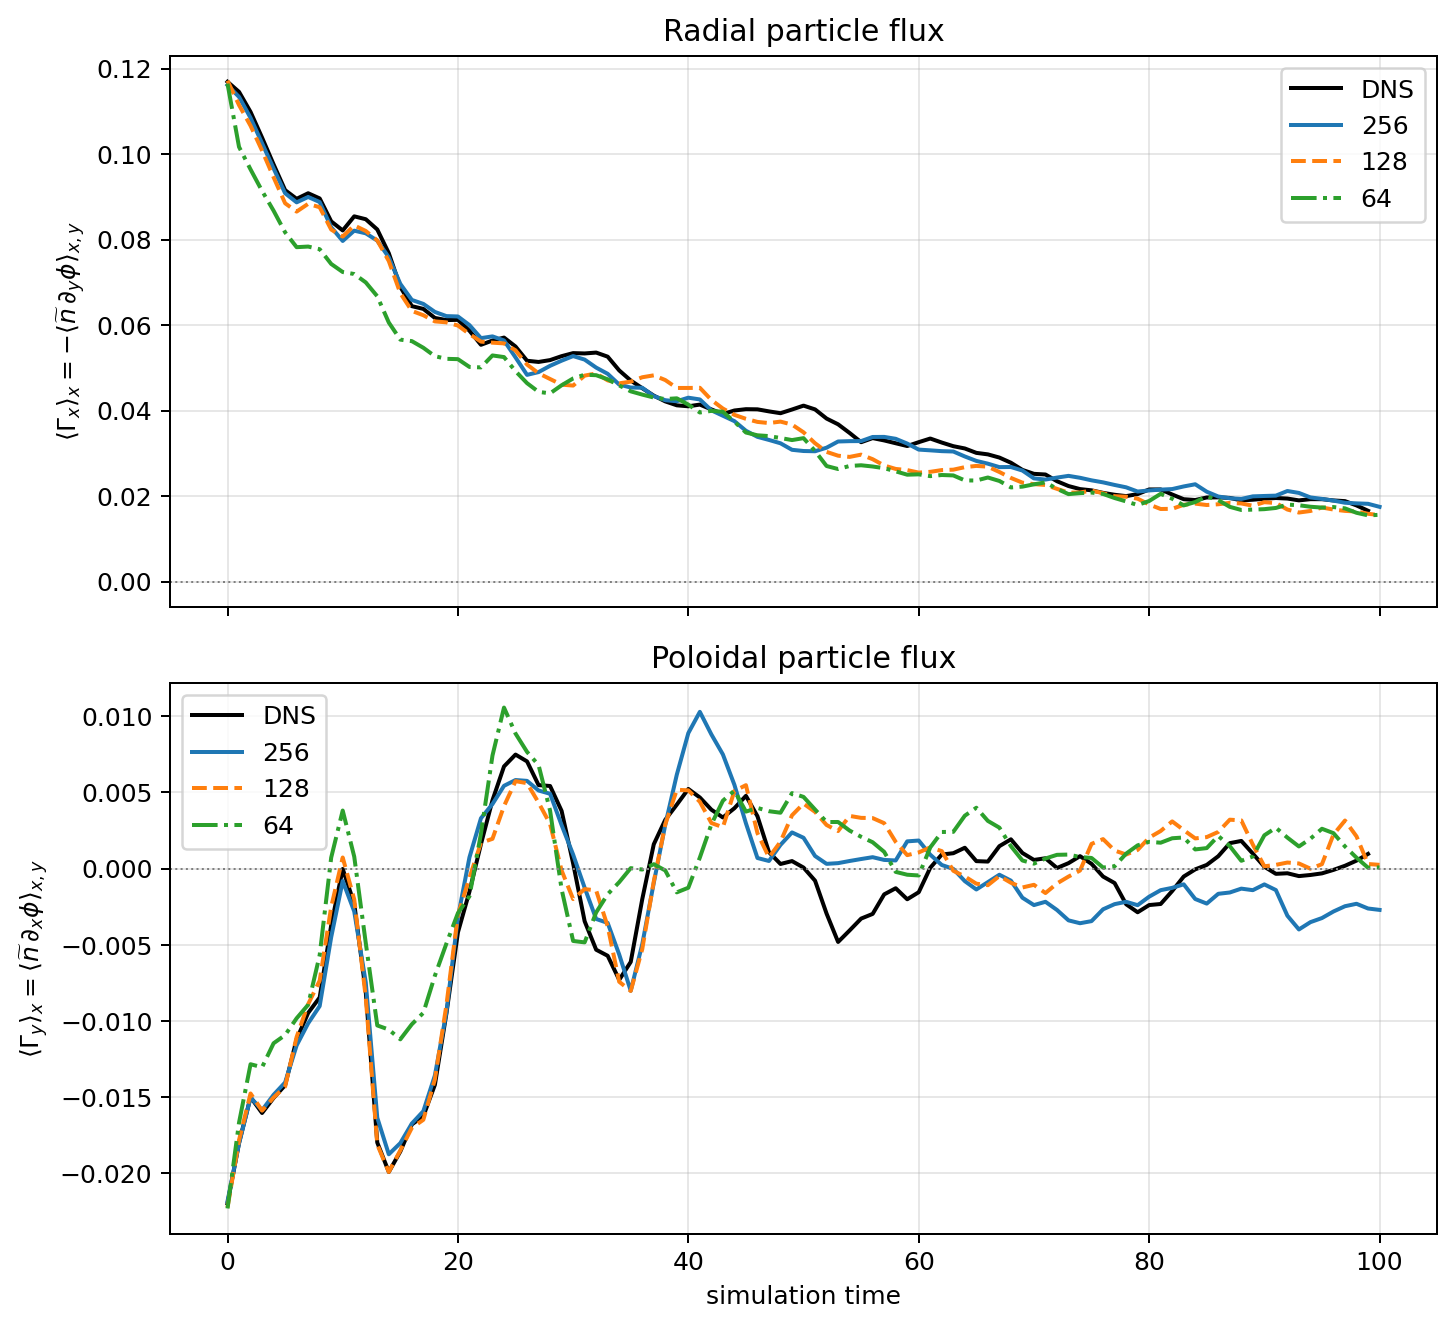
\includegraphics[width=\linewidth]{images/mHW_N512_particle_flux_vs_time.png}
\caption{\texttt{mHW\_N512}}
\end{subfigure}
\caption{Domain-averaged turbulent particle-flux histories. Each case shows radial flux above and poloidal flux below, using the non-zonal density $n'=n-\langle n\rangle_y$. The original plots denote this fluctuation by $\widetilde n$. DNS and reconstruction labels follow the supplied legends.}
\label{fig:particle-flux}
\end{figure}
\subsection{Computational performance}

The computational cost was measured using wall-clock time, CPU/GPU utilization and total number of time steps. The corresponding speedup is
\begin{equation}
    S
    =
    \frac{T_{\mathrm{DNS}}}{T_{\mathrm{AI\text{-}LES}}}.
\end{equation}

\begin{table}[ht]
\centering
\caption{Computational performance.}
\label{tab:performance}
\begin{tabular}{lcccc}
\toprule
Case & DNS time & AI--LES time & Speedup & Memory \\
\midrule
HW\_N256  & TODO & TODO & TODO & TODO \\
HW\_N512  & TODO & TODO & TODO & TODO \\
mHW\_N256 & TODO & TODO & TODO & TODO \\
mHW\_N512 & TODO & TODO & TODO & TODO \\
\bottomrule
\end{tabular}
\end{table}

The principal cost of the proposed method is generator inference. Nevertheless, this cost is offset by the reduced number of spatial degrees of freedom in the LES solver. The measured speedup is [TODO], with the largest benefit observed for [TODO case].

\section{Discussion}

The supplied results assess the evolution of reconstructed-field diagnostics; they do not compare against direct prediction of sub-grid terms. Physical consistency remains an important constraint on the reconstruction. In particular, calculating vorticity from the generated electrostatic potential enforces the elliptic relationship
\[
\zeta=\nabla^2\phi
\]
and prevents independent-field drift.

The modified $256^2$ case highlights a limitation of relying on energy alone: near-DNS energy can coexist with excess enstrophy, altered PDFs and delayed transport bursts. The closer agreement of the modified $512^2$ case applies to a much shorter interval and does not establish improved long-time stability with increasing resolution.

The approach has several limitations. First, the generator may produce nonphysical small-scale structures outside the training distribution. Second, long-time stability is not guaranteed solely by minimizing instantaneous reconstruction error. Finally, the present method is limited by the validity of the chosen filter and by the statistical coverage of the training dataset.

\section{Conclusions}

A generative-AI closure for edge-plasma LES has been developed by learning DNS fields filtered with a Germano-consistent procedure. The reconstructed fields are used to evaluate the nonlinear Poisson-bracket terms, while the vorticity is obtained directly from the generated electrostatic potential.

The method was tested with the HW\_N256, HW\_N512, mHW\_N256 and mHW\_N512 configurations. The main conclusions are:

\begin{itemize}
    \item the generative model reconstructs the dominant spatial structures of the DNS fields;
    \item the learned fields retain several large-scale statistical features, while high-wavenumber spectral tails and late-time mHW\_N256 enstrophy show discrepancies;
    \item radial-flux trends are reproduced in several intervals, but burst timing and poloidal-flux fluctuations differ from DNS;
    \item a measured computational speedup remains to be established;
    \item the mHW\_N256 trajectory exhibits pronounced late-time discrepancies; unequal observation windows preclude a controlled resolution ranking.
\end{itemize}

Future work will investigate parameter-conditioned generators, explicit enforcement of conservation laws, uncertainty quantification and extension to fully three-dimensional edge-plasma models such as Hermes-3.

\section*{Acknowledgements}

The authors acknowledge the use of the BOUT++ framework and computational resources provided by [TODO].

\bibliographystyle{elsarticle-harv}
\bibliography{Paper_3DHW}

\section*{Code and model weights availability}

The source code is available at \url{https://github.com/stfc/U-Net-LES}.
The model weights are available on Zenodo at \url{https://doi.org/10.5281/zenodo.22973917}.

\end{document}
